\part{Des données à valoriser}

\clearpage
\thispagestyle{empty}
\cleardoublepage

\chapter{Données graphiques, données chiffrées}

\section{Le lien entre le texte et les images du texte}

Dans chaque élément \texttt{<facsimile>}, une balise \texttt{<surface>} définit le bloc de segmentation supérieur (la page). L'élément suivant, \texttt{<graphic>}, indique dans son attribut \texttt{@url} la localisation de l'image de la page segmentée. L'ensemble des images étant stocké dans l'espace alloué au programme \timeus{} au sein du service \sharedocs{} de la TGIR Huma-Num, la localisation consiste en un chemin relatif (\fig{} \ref{fig:facsimile} p. \pageref{fig:facsimile}).

Or ces images sont déjà hébergées par \ia. Elles ont été téléchargées sur le \sharedocs{} dans le but de permettre leur segmentation par \textit{FineReader} et \transkribus{} puis leur \ocr{} par \lse. Leur conservation après l'obtention des fichiers XML n'est plus aussi pertinent que celle des prises de vues des registres prud'homaux effectuées dans des dépôts d'archives, qui n'existent sous aucune autre forme. Rappelons également qu'\ia{} se donne pour objectif d’être un centre stable et durable d’archives digitales ; aussi est-il peu probable que les images des \odm{} disparaissent de ses serveurs. Il nous a donc été demandé de substituer le chemin local par l'adresse de l'image sur \ia{} (\ann{} \ref{ann:feuille_route}, \issue{} 2) ; cette mission a donné lieu à la publication d'un billet sur le carnet de recherche du programme \timeus\footcite{genero}.

Nous avons apporté deux solutions : l'une employait les URLs basiques des images, l'autre mobilisait les manifestes \iiif{} des volumes. Toutes deux ont donné lieu à des scripts Python dont les fonctionnements sont similaires.

Les URLs se trouvaient dans des fichiers JSON renseignés dans le code source des pages d'\ia. Un fichier JSON contient des informations représentées de manière structurée ; il s'agissait ici de métadonnées concernant le volume numérisé. Parmi celles-ci, une sous-section intitulée \texttt{data} contenait des métadonnées (longueur, largeur, etc.) et l'URI de chaque image. Ces images étaient au format JPEG et correspondaient à celles déposées sur le \sharedocs. 

Le problème posé par cette solution est que les adresses n'étaient pas stables. En effet, au bout d'un certain temps, elles ne fonctionnaient plus car les informations avaient changé dans le fichier JSON source.

Aussi avons-nous exploré la piste du \iiif. L'\textit{International Image Interoperability Framework} permet d'afficher une image avec ses métadonnées dans le contexte d'une application web directement depuis le serveur où elle est stockée (ici, \ia). Les URLs de cette deuxième solution se trouvent dans les \og manifestes \iiif{} \fg{} des volumes : il s'agit des documents JSON contenant leurs métadonnées et référençant les points d'accès aux images (\cad{} leurs URIs dans le protocole \iiif).

Si ces images possèdent le même format que celles de la première solution, leur qualité est bien supérieure et permet d'effectuer des agrandissements d'une très grande profondeur. Du reste, le \iiif{} permet également de naviguer dans un volume en passant de page en page. Cette seconde solution est ainsi plus intéressante pour le projet \timeus{} dans la mesure où elle lui permet d'accéder d'une manière relativement simple à un document contenant un ensemble de données et de métadonnées qui pourront être valorisées au moment d'une édition en ligne.

Le script dont il est ici question, s'il se limite à insérer les URIs des images dans le code XML, commence par effectuer une requête pour lire le contenu des manifestes \iiif{} des \odm{}. Pour cela, il lit un CSV où nous avons enregistré les identifiants donnés par \ia{} aux numérisations, et les utilise pour compléter l'adresse des manifestes (\texttt{https://iiif.archivelab.org/iiif/<itemid>/manifest.json}). Ces lignes de code peuvent être réutilisées, probablement sous la forme d'une fonction, pour obtenir tout type de métadonnées issues des manifestes. En plus de rationaliser le stockage sur le \sharedocs{}, ce script prépare donc l'étape de la publication en ligne.

\section{Les données graphiques dans le flux textuel}

Un des principaux apport du \iiif{} pourrait être le traitement des objets graphiques qui, nous l'avons vu, sont nombreux dans les pages des \odm{} (\fig{}~\ref{fig:ex_figures} p. \pageref{fig:ex_figures}). En particulier, les photographies, les figures ou les cartes pourraient bénéficier des fonctionnalités d'agrandissement afin de permettre à l'utilisateur de pleinement les prendre en considération.

Pour rendre cela possible, il faudrait disposer d'une évaluation du taux de détection des figures. Ce chiffre n'est pas connu, mais des relevés aléatoires laissent penser qu'il risque d'être inférieur à 60\%. Les tableaux sont les figures qui ont posé le plus de problème au script, nous y reviendrons.

Parmi les autres, plusieurs n'ont été que partiellement détectées. La carte de la page 439 de la monographie \no{} 90\footcite{mono090a} est ainsi parfaitement détectée et transposée dans un élément \texttt{<figure>} (\fig{} \ref{fig:odmfig90439}). À l'inverse, le plan d'une \og habitation cambodgienne à Pnom-Penh \fg{} est détecté en double --- peut-être en raison de la superposition d'une vue de face de l'habitation et de son plan --- et le titre de la figure est transcrit comme du texte (\fig{} \ref{fig:odmfig90453}). Dans la monographie suivante\footcite{mono090b}, la photographie pleine page \og Cambodgiens et amanites \fg{}, insérée entre les pages 484 et 485, a été retirée du texte et n'est pas présente dans les fichiers sous quelque forme que ce soit.

\begin{figure}
    \centering
    \begin{subfigure}{0.4\textwidth}
     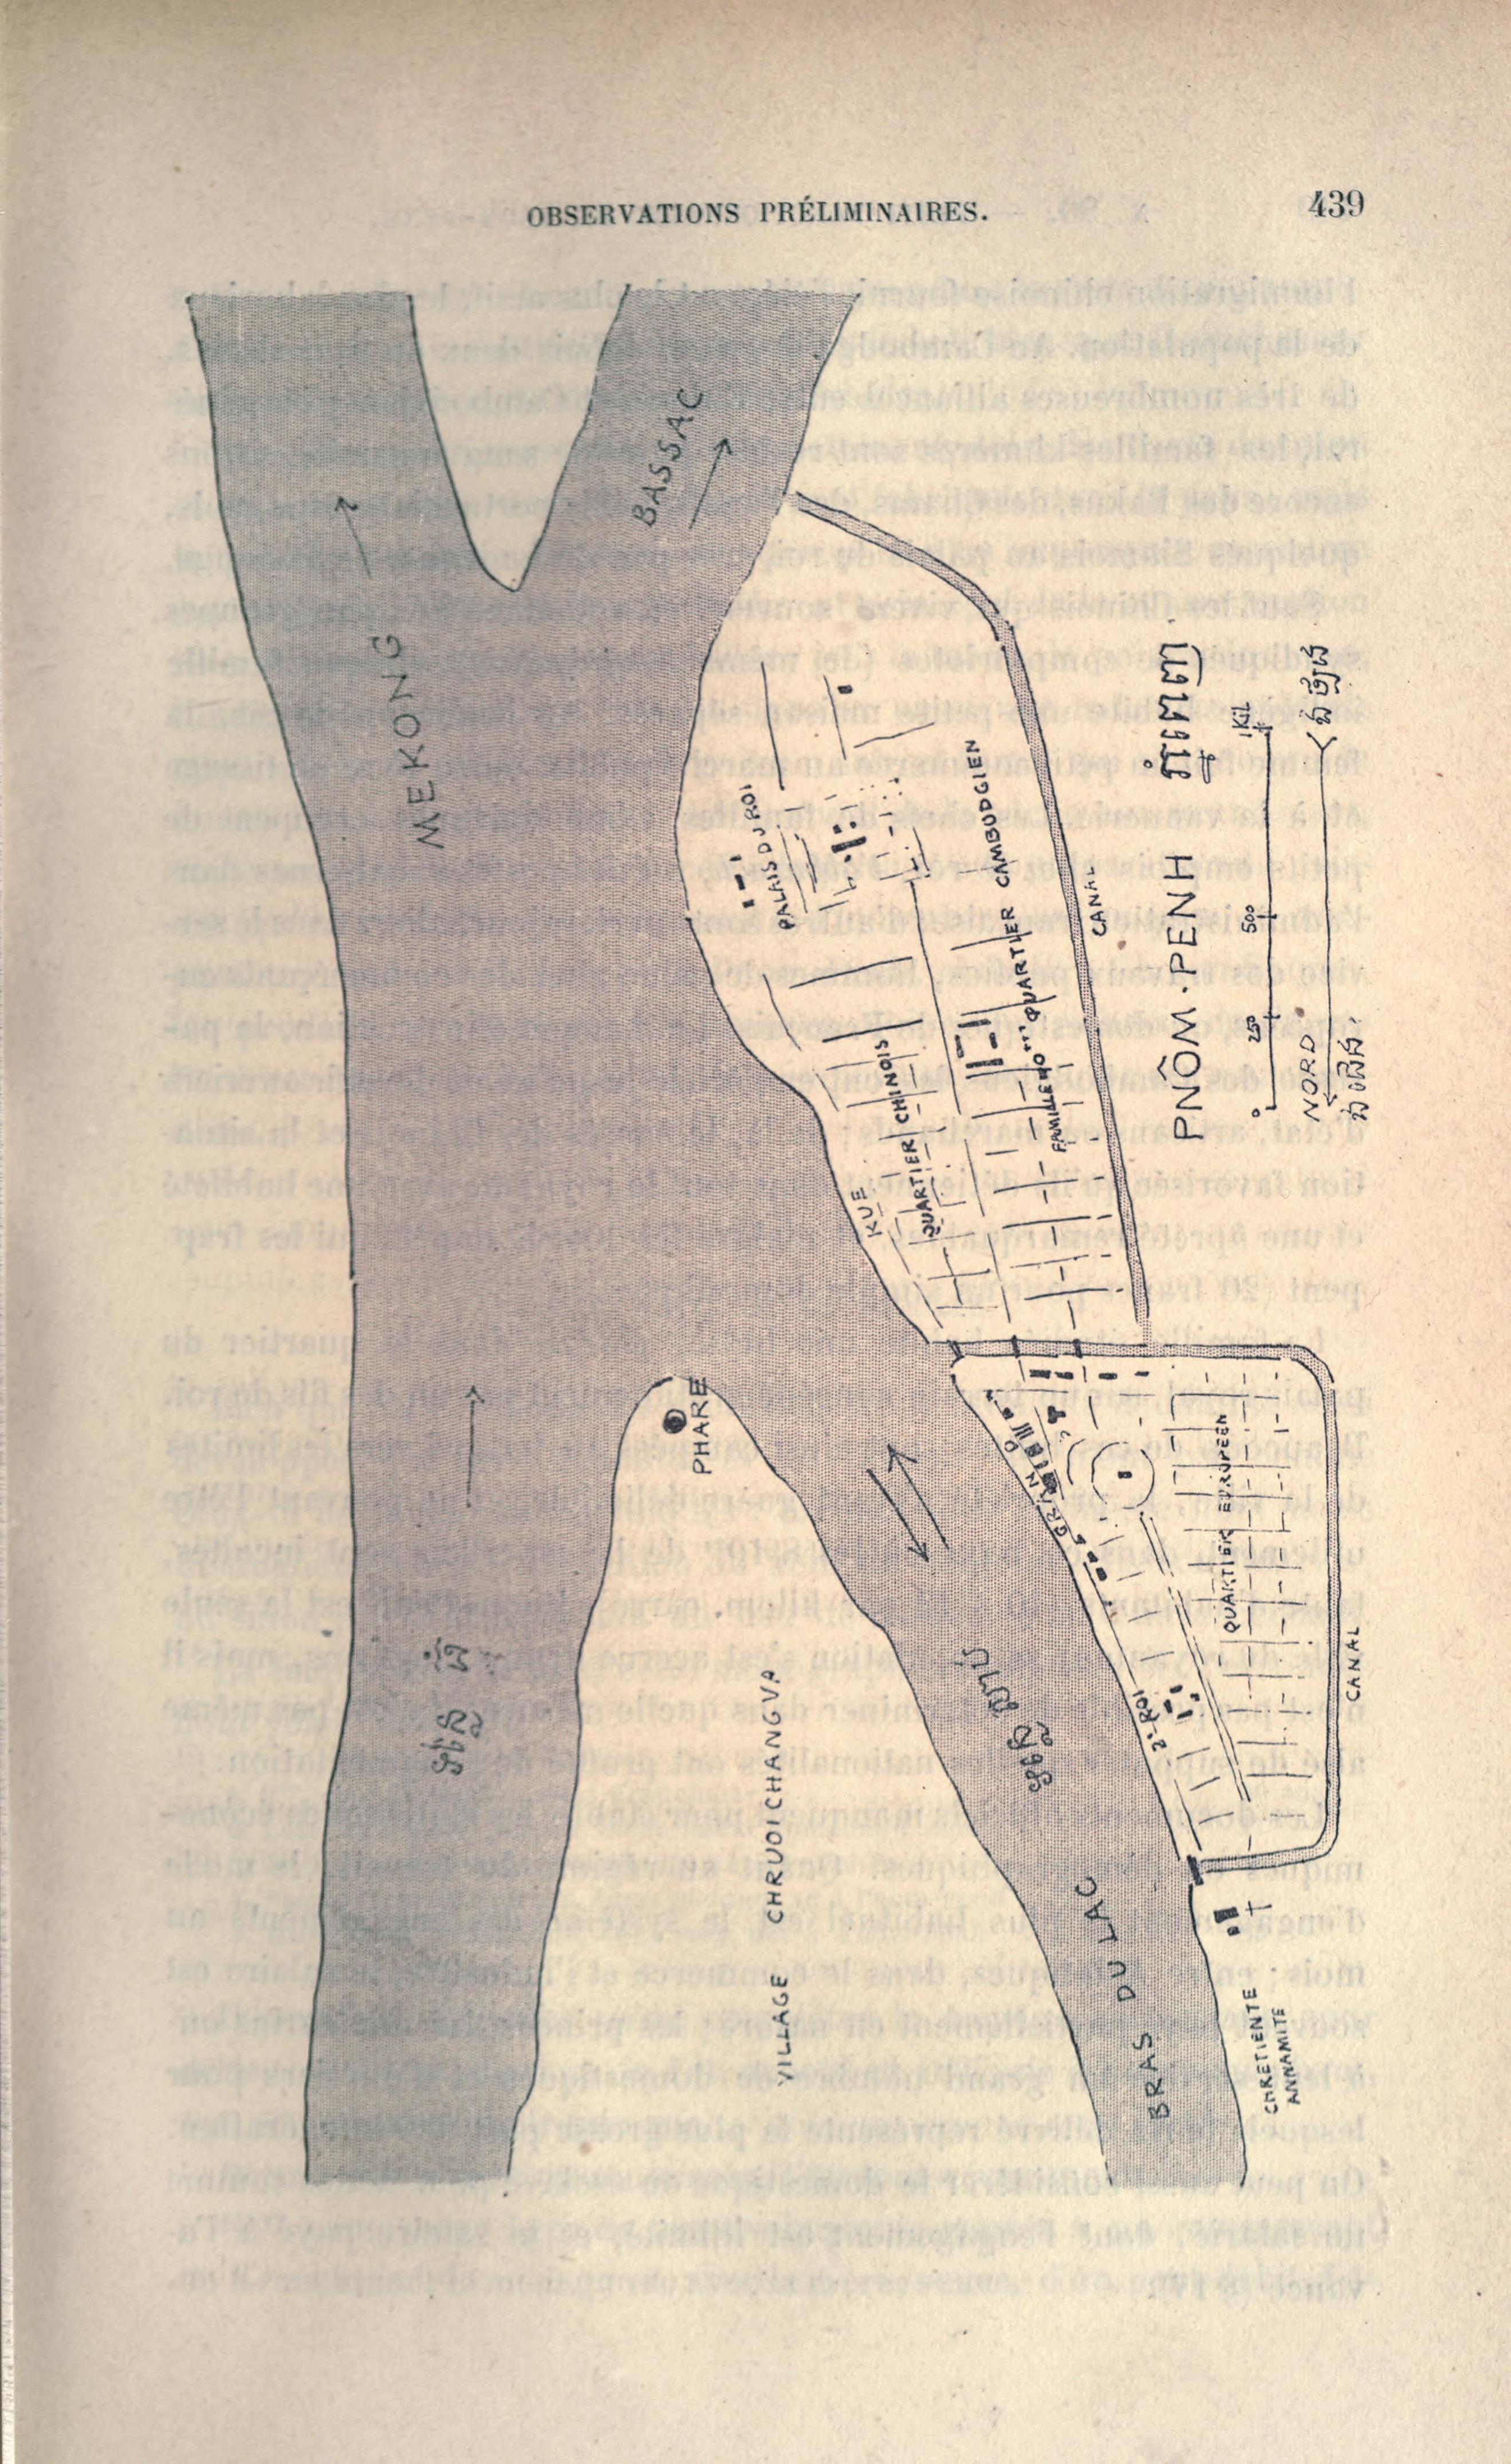
\includegraphics[width=1\linewidth]{img/odm90_439.jpg}
     \caption{Page 439 : détection optimale de la carte.}
     \label{fig:odmfig90439}
    \end{subfigure}
    \hspace{5pt}
    \begin{subfigure}{0.4\textwidth}
     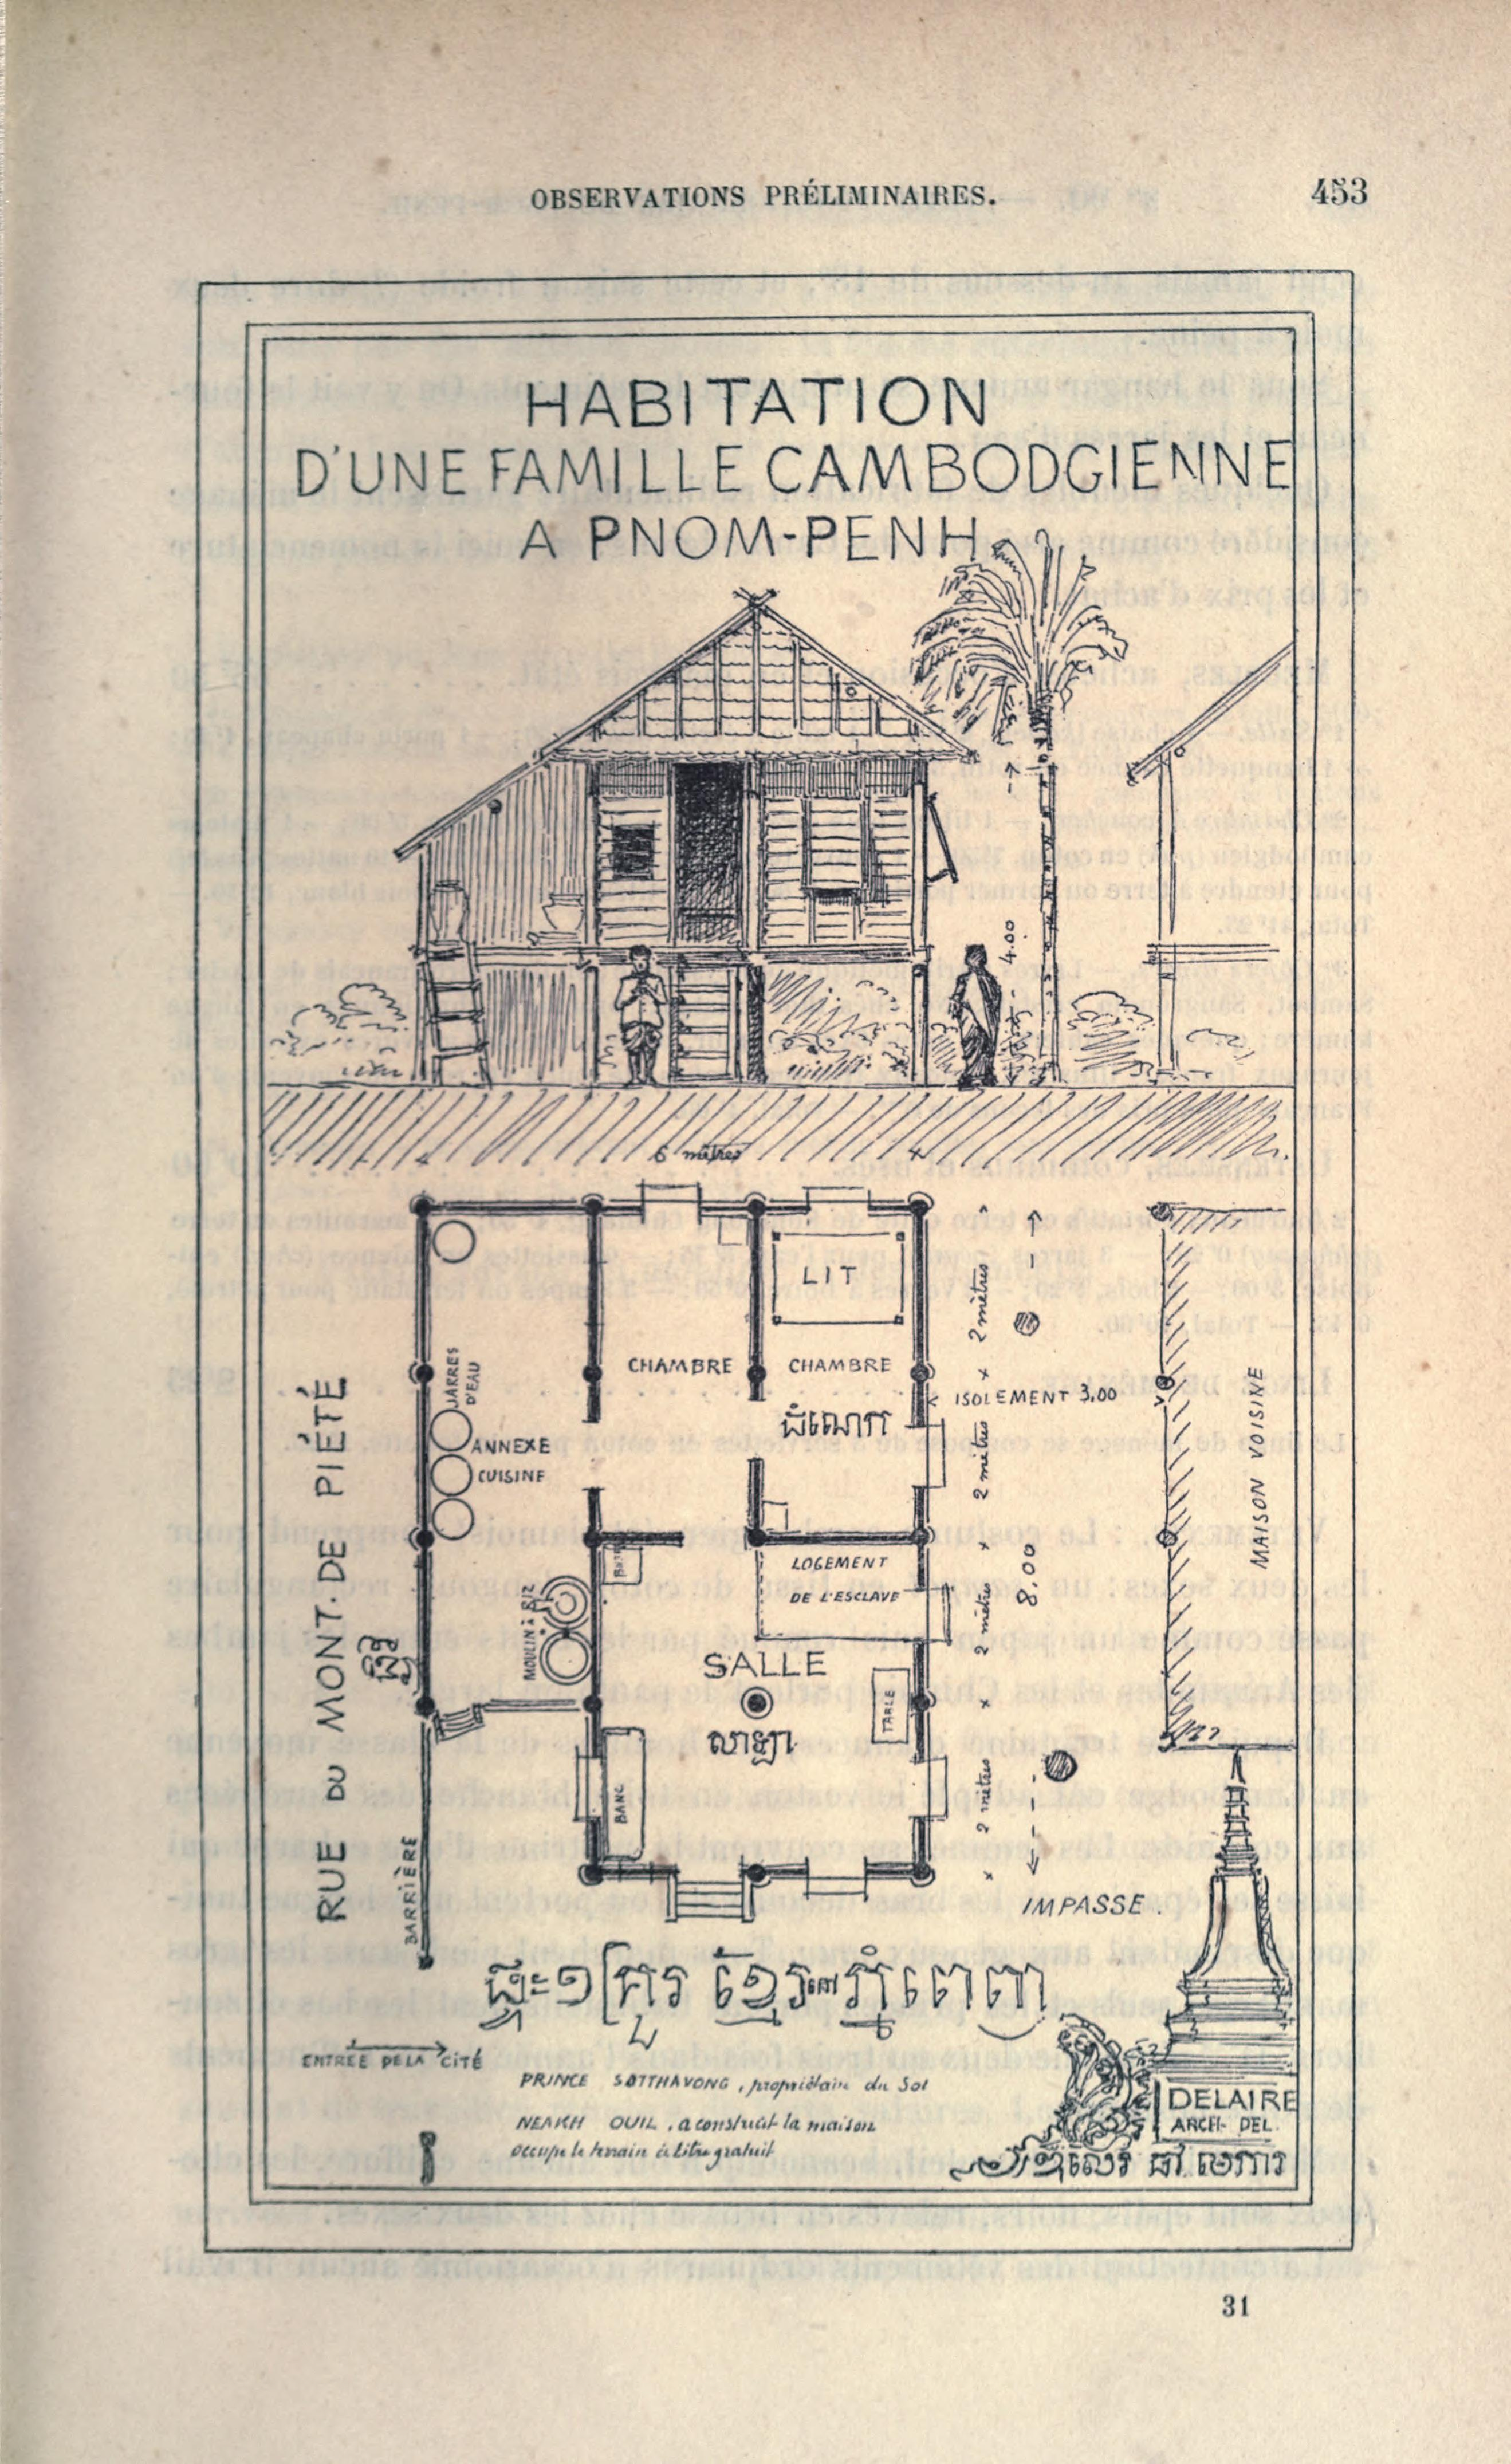
\includegraphics[width=1\linewidth]{img/odm90_453.jpg}
     \caption{Page 453 : détection en double et transcription du titre.}
     \label{fig:odmfig90453}
    \end{subfigure}
    \caption{Figures dans la monographie \no{} 90.}
    \label{fig:odmfig90}
\end{figure}

Ces erreurs de détection ne peuvent pas être résolues de manière automatique : aucune table des figures n'est présente dans les volumes. Un tel outil eut permis de cibler les pages à contrôler et de ne pas avoir à chercher visuellement les figures. Une intervention manuelle, possiblement longue, s'impose donc.

La présence de ces figures est également un élément à garder à l'esprit au moment de la reconstitution des paragraphes. En effet, certaines sont insérées en plein milieu de ces derniers. Pour ne pas perturber la reconstitution, il sera nécessaire d'ajouter une condition spécifiant que les balises \texttt{<p>} commençant pas une minuscule ne constituent pas une unité indépendante, et ce même si elles sont précédées d'une figure. Le problème de cette méthode est qu'elle présuppose que \lse{} a bien fait la différence entre une majuscule et une minuscule en début de phrase, ce dont on ne peut pas être totalement certain.

Ajoutons enfin que les figures de type carte, croquis ou photographie ont une importance relative du \pov{} de la donnée pure. Elles ne sont pas utiles aux chercheurs et aux chercheuses qui s'intéressent au vocabulaire du textile ou du monde ouvrier, ni à ceux qui souhaitent recueillir des données chiffrées. Dans le document XML, elles ne sont que des repères dont la nécessité ne se révélera qu'au moment de la transformation des fichiers pour une interface de visualisation.

\section{Les tableaux : images ou données ?}

À l'inverse, les tableaux qui jalonnent le corpus ont une importance considérable en raison des informations statistiques qu'ils contiennent. Plus particulièrement, les budgets des paragraphes 14 à 16 constituent \og la pièce centrale \fg{} des monographies leplaysiennes\footcite[p. 317]{savoyecontinuateurs}. Les \textit{Observations préliminaires} sont en effet entièrement tournées vers leur établissement ; le monographe n'arrête son enquête que lorsqu'il a établi un budget équilibré offrant une vue globale des recettes et des dépenses de la famille. En effet, dans la démarche de Frédéric Le Play, \og l'argent est pris comme unité de mesure de la vie sociale, le budget étant la quantification, en termes de revenus et dépenses, de l'ensemble des activités de la famille \fg\footcite[p. 317]{savoyecontinuateurs}.

D'un \pov{} technologique, il n'est cependant pas simple de reproduire à l'identique ces tableaux. La TEI comporte un ensemble de balises destiné à cet effet --- \texttt{<table>}, \texttt{<row>} et \texttt{<cell>} --- mais le problème est ici fonction de la segmentation et de la compréhension par un script de la mise en page du tableau. Or cette mise en page peut se révéler sophistiquée. Ainsi, le texte est centré lorsqu'il s'agit de titre d'article ou de section, aligné à droite pour les postes de dépenses ou les recettes, aligné à gauche pour le total. Lorsque plusieurs postes de dépense successifs partagent une même formulation dans leurs intitulés, celle-ci n'est pas répétée mais signifiée par des traits de rappel.

Ces modulations permises par l'imprimé ne sont pas envisageables dans un tableau numérique, où toute donnée chiffrée doit correspondre à un libellé défini et non suggéré afin d'être rendu exploitable. Face à ce type d'information, un algorithme idéal devrait être capable de reproduire le processus cognitif de reconstruction effectué par le cerveau humain. En l'état actuel de l'avancée technique, faire en sorte que la machine différencie un trait de rappel d'une ligne de séparation entre deux cellules n'est pas aisé. Cela constitue un sujet de recherche à part entière et ne peut pas être mené dans le temps imparti par l'ANR au programme \timeus.

Le traitement des tableaux doit donc être pensé à l'aune de ces difficultés techniques et temporelles. Dans un essai de mise en scène des fichiers XML au format HTML, Alix Chagué a ainsi choisi de transformer les balises \texttt{<figure>} --- signifiant notamment la présence des tableaux --- en des icônes cliquables qui redirigent vers les images des pages où ces figures se trouvent. Le procédé est habile mais se fonde sur l'idée que toutes les figures ont été détectées, ce qui n'est pas encore le cas. Du reste, cela ne permet pas d'exploiter directement les informations des tableaux.

Pour autant, cette idée du tableau comme une image est sérieusement étudiée par le programme \timeus. L'effort d'ingénierie d'études se concentrerait alors sur la modélisation et l'implémentation d'une indexation fine des différents tableaux.

Il serait tout d'abord nécessaire d'effectuer un recensement exhaustif des tableaux des \odm. Ensuite, une étape de modélisation commencerait par l'analyse de leur structuration afin de faire ressortir les points communs et \textit{in fine} de constituer des catégories ; en parallèle, les chercheurs et les chercheuses devront définir leurs besoins -- sont-ils intéressés par l'ensemble des informations, ou bien seules celles ayant trait au textile ? Une fois la typologie arrêtée et les besoins déterminés, il sera possible d'envisager l'implémentation d'une nouvelle couche d'encodage scientifique dans les fichiers XML.

Celle-ci pourrait se traduire par deux actions. D'une part, un identifiant \texttt{@xml:id} pourrait être donné à chaque titre de paragraphe, et ensuite référencé dans un attribut \texttt{@ana} (\texttt{analytic}). Peu intéressants pour les paragraphes de budget qui contiennent systématiquement des tableaux, ces attributs permettraient de signaler ceux que l'on peut rencontrer dans les paragraphes 6 à 10 (\textit{Propriétés}, \textit{Subventions}, \textit{Travaux et industries}, \textit{Aliments et repas}, \textit{Habitation, mobilier et vêtement}). D'autre part, un recensement des objets des tableaux --- dépenses de nourriture, dépenses pour l'habitation, dépenses pour le textile, etc. --- pourrait fournir une liste de valeurs pour un attribut \texttt{@type}. Au-delà de permettre un traitement rationnel des tableaux au regard des impératifs scientifiques et temporels, cette méthode pourrait servir de base à l'établissement de vues logiques ou de facettes de recherche conduisant à l'affichage des tableaux sur une base thématique.

La valorisation des objets graphiques n'est donc pas chose aisée. Elle peut se restreindre à leur simple reproduction doublée d'une indexation qui, si elle oriente le chercheur, ne le dispense pas d'effectuer lui-même l'extraction des données chiffrées ou textuelles contenues dans la figure. Il y a ici une limite au projet de numérisation du corpus.

\newpage
\thispagestyle{empty}
\mbox{}
\newpage

\chapter{Données textuelles, données scientifiques}

\section{La qualité de l'\ocr}

L'extrême majorité des données des \odm{} est composée de texte. Ce texte peut être le support de différentes études, qui se basent toutes sur la lecture. La lecture par l'\oe{}il humain --- le corpus n'est pas réellement important et un chercheur ou une chercheuse peut en prendre intégralement connaissance ---, mais aussi la lecture par une machine, \cad{} l'analyse automatique. Ces deux opérations ne nécessitent pas un même niveau de qualité de l'\ocr{} et ne s'adressent pas au même public --- la première est accessible à un large groupe, la seconde requiert l'assistance technique d'un ingénieur et l'exécution par une machine.

La qualité d'une \ocr{} peut être mesurée par différents indices, au niveau du caractère (\textit{character error rate}, CER) ou du mot (\textit{word error rate}, WER).  Le CER est obtenu grâce la formule suivante :

\[CER = \frac{S + D + I}{N}\]

où \textit{S} représente le nombre de substitutions (caractères dont la reconnaissance n'est pas correcte), \textit{D} le nombre de suppressions (\textit{deletions}), et \textit{I} le nombre d'insertions, \cad{} les caractères qui ne sont pas présents dans la vérité terrain que l'on trouve pourtant dans l'\ocr. La somme de ces trois chiffres est divisée par le nombre total de caractères dans le fichier de vérité terrain (\textit{N}).

À partir d'une vérité terrain de 1300 lignes, Alix Chagué avait calculé un CER de 2,2\% pour l'\ocr{} des \odm\footcite[slide 16]{inria-pp}. Ce taux très faible est le signe d'une transcription de bonne qualité. Où se situent les erreurs restantes ?

Dans les \odm{} comme dans de nombreux autres corpus\footcite[p. 1]{sagot}, elles se concentrent sur les entités nommées. Au premier rang de ces dernières figurent les patronymes et les toponymes (\fig{} \ref{fig:mono-56-page-4-code}); les \og expressions temporelles et les expressions de quantité \fg{} ou encore \og les nombres, les formules chimiques, les unités monétaires \fg{} sont également concernés\footnote{Les entités nommées sont définies dans le domaine du traitement automatique du langage comme des \og unités faisant référence à une entité unique et concrète et réalisées par des noms propres (noms de personnes, d’organisations, d’artefacts ou de lieux) \fg{} : \cite[p. 4]{sagot}}. Ces entités sont très peu représentées dans les fichiers de vérité terrain sur lesquels le logiciel s'entraîne ; pour augmenter leur détection, un entraînement spécifique et focalisé serait nécessaire.

\begin{figure}[ht]
    \centering
    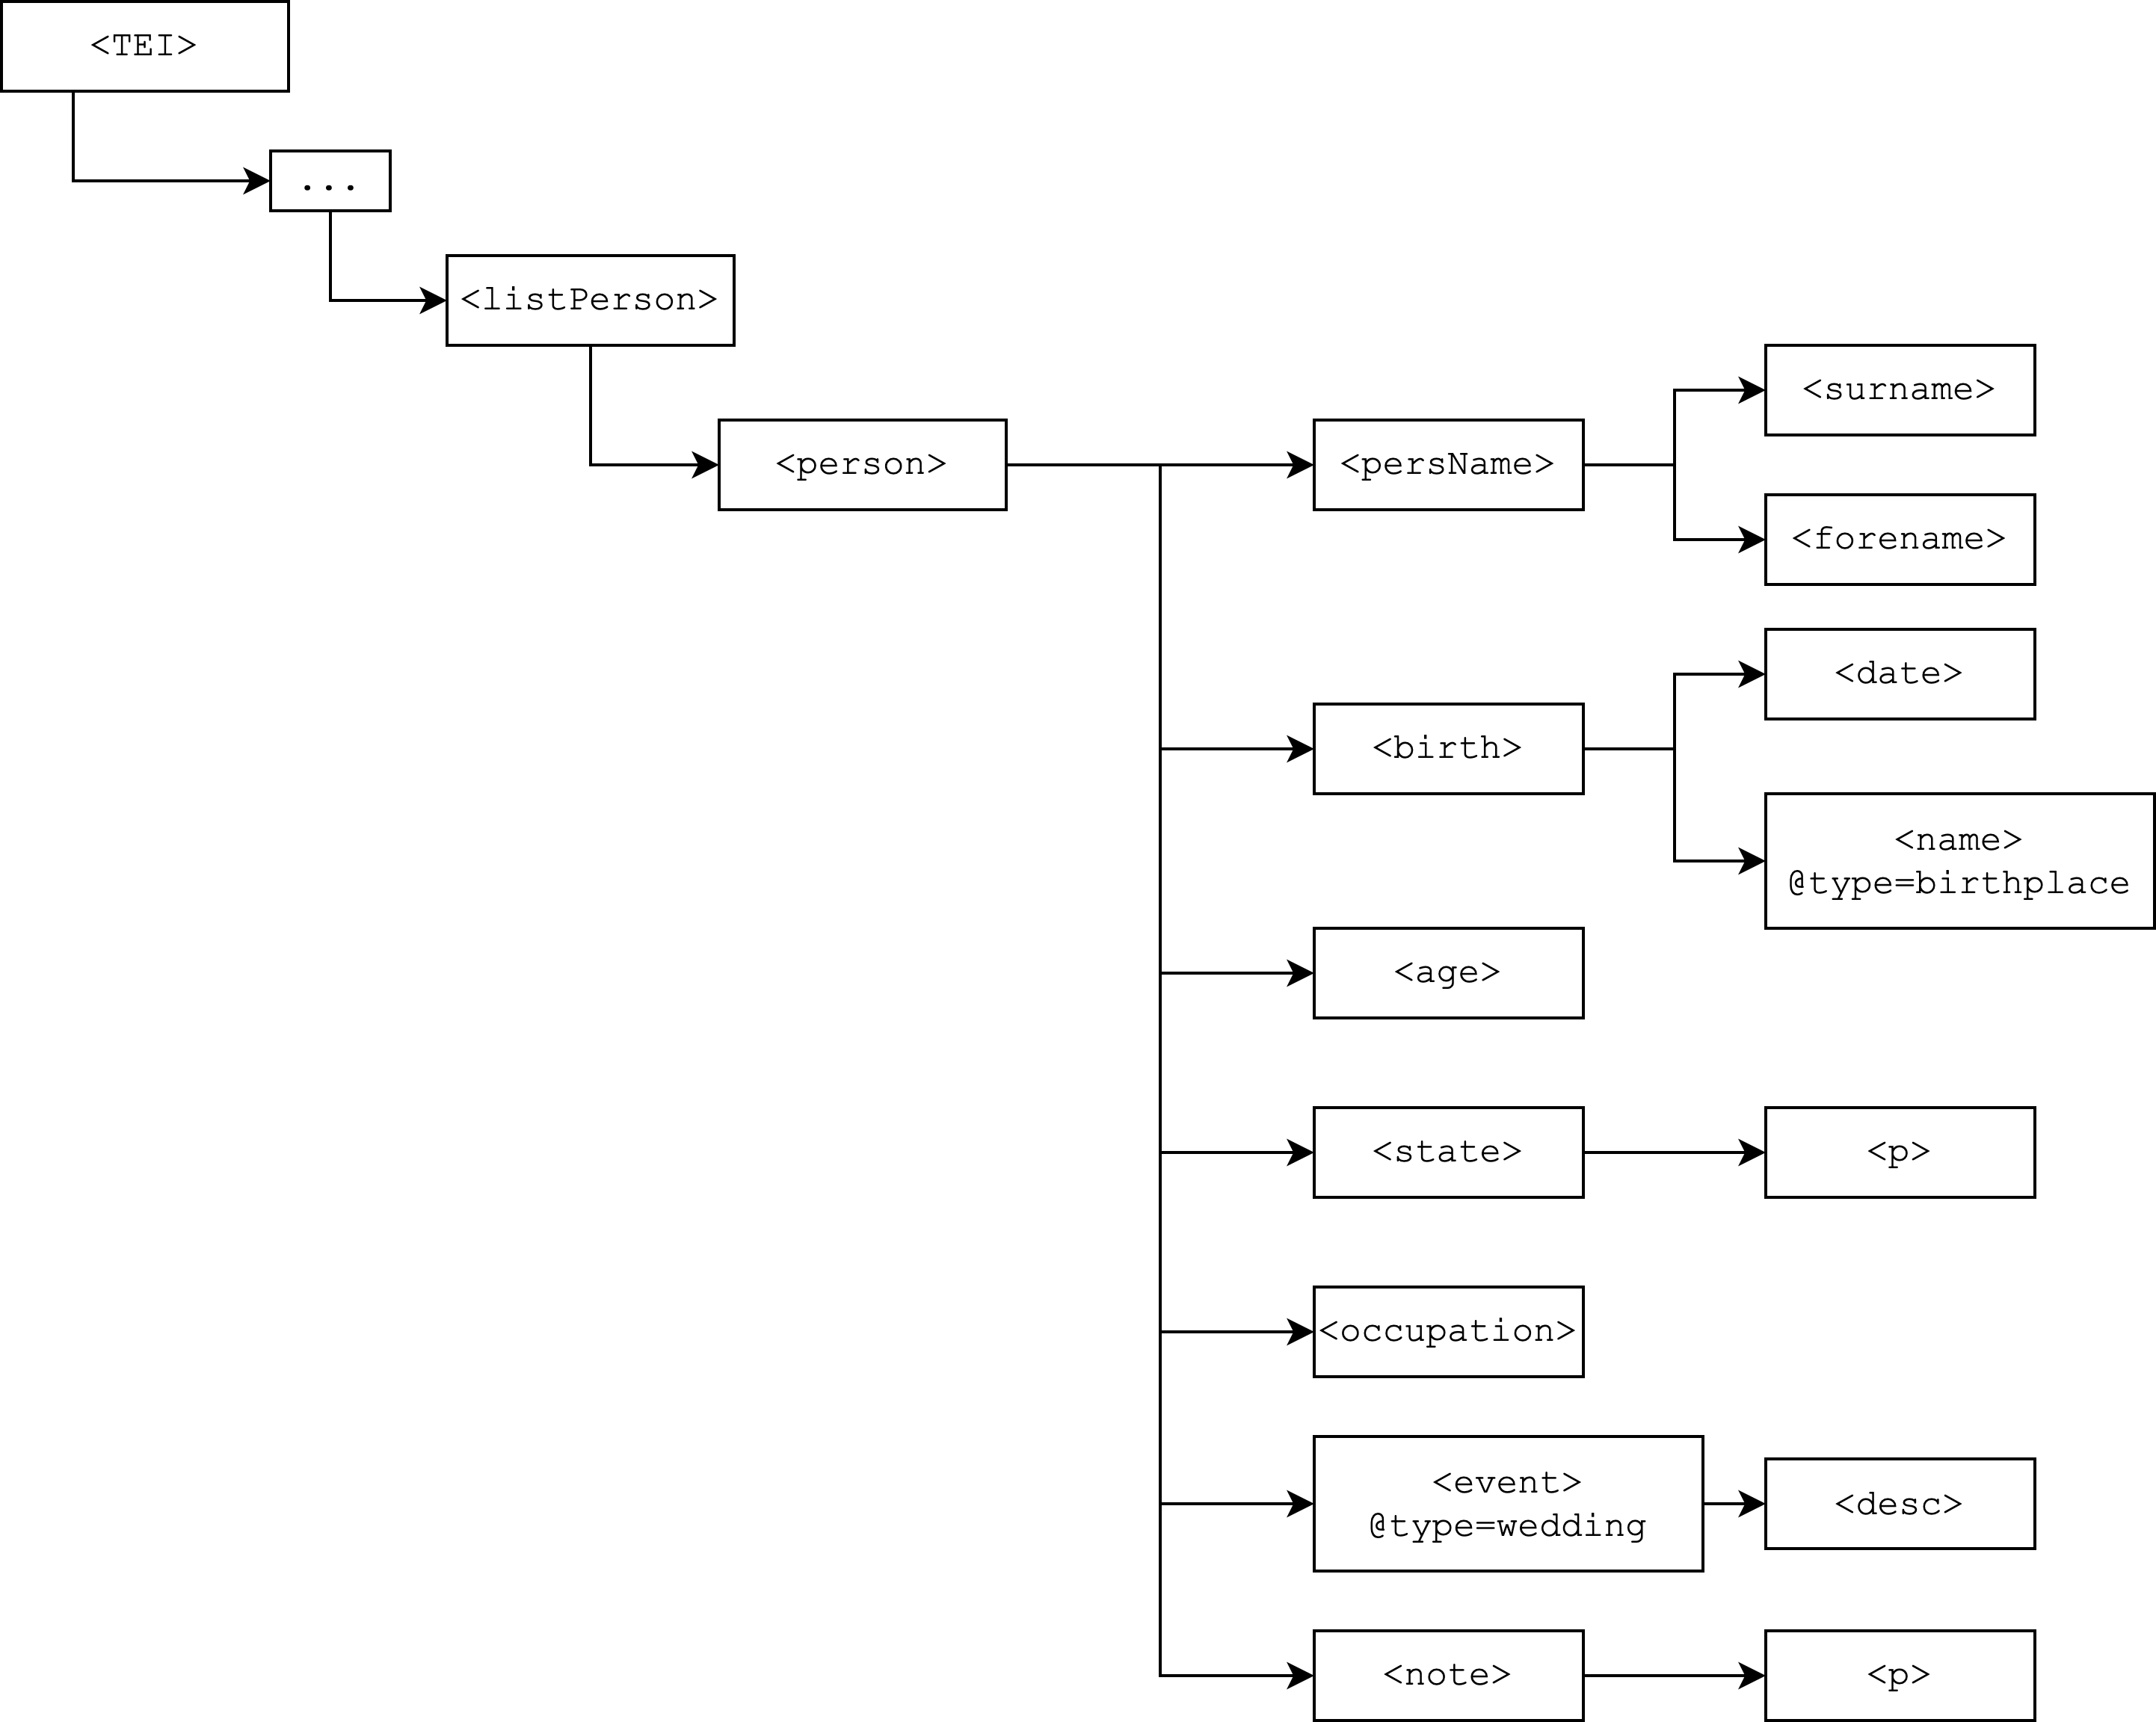
\includegraphics[width=16cm]{img/schema_index.png}
    \caption{Arbre XML simplifié montrant l'organisation d'une entrée d'index.}
    \label{fig:index_tree}
\end{figure}

\section{Indexer les individus}


Cette défaillance dans la détection des entités nommées pose problème dans la mesure où les monographies de familles prennent pour sujet un groupe d'individus (les enquêtés) sur un territoire précis ; si leurs noms sont souvent anonymisés (\textit{M***}, \textit{F***}, etc.), les prénoms sont écrits en toute lettre.

Un projet de recherche mené par le CMH et le CHR concerne ces enquêtés et souhaite les indexer en relevant les informations biographiques données par les monographes. Ce travail d'indexation des familles enquêtées est mené par Alain Cottereau et Stéphane Baciocchi (CRH, EHESS), avec Anne Lhuissier (CMH, INRAE). Ils  cherchent notamment à lever l'anonymat  des individus et à compléter (voire corriger) les informations biographiques délivrées dans les monographies, grâce à l'exploitation des fonds d'archives départementaux ou municipaux.

Anne Lhuissier et Stéphane Baciocchi se sont ainsi rendus aux Archives départementales de l'Isère pour trouver des informations sur le gantier Théodore  G., sujet principal de la monographie \no{} 55\footcite{mono055a}. Théodore  G. est présenté comme un gantier vivant à Biviers, à 9km de Grenoble. Son père, mort avant le début de l'enquête, était un riche cultivateur ; les frères de Théodore cultivent toujours, au moment de l'enquête, les terres familiales. Le monographe explique que Théodore, doté \og d'une forte constitution \fg{}, a lui-même \og pris part jusqu'à l'âge de vingt-cinq ans aux travaux de l'agriculture \fg{}\footcite[p. 471]{mono055a}.

Son service militaire l'amène ensuite à participer au siège de Sébastopol lors de la guerre de Crimée en 1855\footcite[p. 471]{mono055a}. Cependant, son père \og l'a racheté et rappelé auprès de lui \fg{}, \cad{} qu'il a payé un remplaçant qui a effectué la fin de son service militaire à sa place\footcite[p. 471]{mono055a}. C'est alors que, en dépit du fait qu'il \og passait à juste titre pour un des ouvriers les plus intelligents et les plus certains de réussir \fg{} dans l'agriculture, relate le monographe, \og il n'a pu résister au désir d'apprendre la profession de gantier \fg{}\footcite[p. 471]{mono055a}. Théodore est ainsi le seul homme de sa fratrie à ne pas être devenu agriculteur.

Or Anne Lhuissier et Stéphane Baciocchi, en exploitant les archives des séries \textsc{e} (archives notariales), \textsc{p} (cadastre) et de la sous-série \textsc{3q} (enregistrement et timbre), ont pu démontrer que Théodore avait reçu une part si faible de la succession paternelle, qu'il n'était pas envisageable pour lui de poursuivre dans l'agriculture. Ses frères avaient en effet fait valoir que le paiement d'un remplaçant pour son service militaire devait être considéré comme une avance sur l'héritage, et donc déduit de celui-ci. Théodore n'a reçu aucune partie des terres paternelles mais seulement une maison ; Anne Lhuissier et Stéphane Baciocchi font l'hypothèse que cette absence de terre à cultiver a été déterminante dans sa volonté de devenir ouvrier et donc de rompre avec le travail traditionnel de sa famille\footnote{Ces lignes sont écrites avec l'aimable autorisation d'Anne Lhuissier et de Stéphane Baciocchi ; leurs conclusions, encore inédites, devraient donner lieu à une prochaine publication.}. Cet exemple illustre les possibilités de valorisation que le programme \timeus{} envisage pour les enquêtés des \odm.

Une tableau prosopographique au format CSV était déjà établi au moment de notre stage. Huit cent quarante-deux individus y étaient identifiés et décrits selon leur état civil et des critères sociaux. Les chercheurs et les chercheuses nous ont demandé de procéder, dans un premier temps, à la transformation de ce tableau en un  index XML et, dans un second temps, à la liaison entre chaque entrée et l'individu correspondant dans les monographies (\ann{} \ref{ann:feuille_route}, \issue{} 4). Du point de vue de l'ingénierie, cela se traduisait par la constitution automatique de l'index puis par l'implémentation dans les fichiers TEI des identifiants des individus cités dans le deuxième paragraphe.

Un fichier d'index au format XML repose sur un \texttt{<body>} dans lequel une ou plusieurs listes de personnes (\texttt{<listPerson>}) sont établies, les individus y étant indexés au sein d'éléments \texttt{<person>}. Nous avons constitué une liste de personnes unique, car aucun besoin particulier ne nous a été transmis quant à cette fonctionnalité de la TEI. On pourrait néanmoins imaginer des listes en fonction des sexes et, à l'intérieur de celles-ci, des sous-listes relatives aux rôles sociaux des individus. 

Nous nous sommes concentrés sur les différentes catégories à faire figurer dans l'index et sur les balises pouvant les traduire (\fig{} \ref{fig:index_tree}).

L'identifiant de l'individu --- formé de celui de la monographie, de la lettre \textit{E} pour \textit{enquêté} et du numéro d'apparition --- constitue la valeur de l'attribut \texttt{xml:id} de la balise \texttt{<person>}. L'état civil se trouve ensuite dans un ensemble \texttt{<persName>} où le nom figure dans \texttt{<surname>} et le prénom dans \texttt{<forename>}.

D'autre balises pourraient venir compléter cette section, notamment \texttt{<addName>} pour les surnoms ou les prénoms surnuméraires. Une reprise du tableau serait néanmoins nécessaire pour rendre l'usage de cet élément possible : dans l'état actuel, le surnom ou le second prénom se trouvent dans la même cellule que le prénom, ici entre parenthèses, là après un tiret et ailleurs introduits par le transitif \textit{dit}. Une telle reprise, consistant donc à répartir en trois cellules (prénom, prénom surnuméraire, surnom) les informations contenues en une pourrait être réalisée sur la plate-forme \textit{Dataiku} qui permet la manipulation de données à grande échelle, par exemple grâce à des expressions régulières.

Les informations de naissance (date et lieu) sont placées dans un ensemble \texttt{<birth>}, suivi de l'âge (\texttt{<age>}).

La situation matrimoniale est décrite par la balise \texttt{<desc>} dans un ensemble \texttt{<event>} (évènement). La TEI conseille de décrire l'évènement de manière normalisée par un \texttt{<label>} placé avant \texttt{<desc>}. Cependant, dans la mesure où cet index ne compte qu'un seul évènement, nous avons choisi de simplifier la structure et d'en préciser la nature grâce à un attribut \texttt{@type} au niveau de \texttt{<event>}. Suivent deux indicateurs contenant le positionnement de l'individu dans la cellule familiale (\texttt{<state>} : chef de famille, femme, fille) et son activité, qu'il s'agisse d'un apprentissage, d'un métier ou d'un travail à la tâche ou à la journée (\texttt{<occupation>}). Dans une \texttt{<note>} finale figurent la date de référence pour les calcules des dates de naissance et de mariage et le rappel du titre de la monographie où apparaît l'individu.

\section{Corriger les transcriptions ?}

Dans chaque volume, le paragraphe \og État civil de la famille \fg{} commence par une liste standardisée des membres de la famille. Les figures \ref{fig:mono-56-page-4} et \ref{fig:mono-56-page-4-code} montrent une comparaison entre le texte d'origine de la monographie 56, sa transcription et son encodage par \lse\footcite[p. 4]{mono056a}. Les erreurs concernant la reconnaissance des entités nommées y apparaissent clairement : sur quatre prénoms, tous sont transcrits avec une distance d'édition importante et le nom de famille \og B*** \fg{} n'est absolument pas reconnu.

\begin{figure}[ht]
    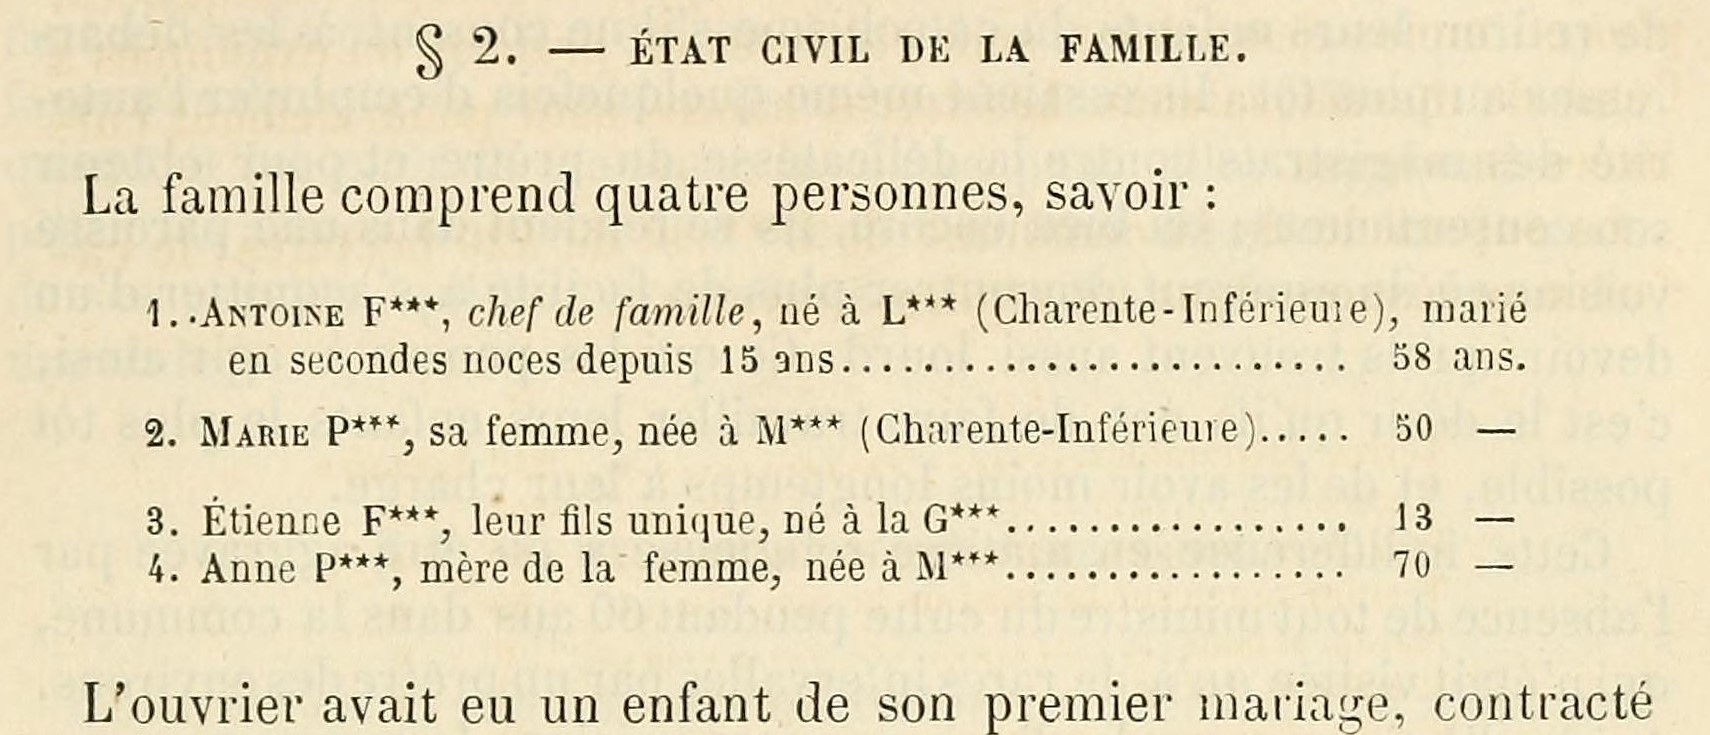
\includegraphics[width=14cm]{img/mono-23-page-209.jpg}
    \caption[Liste d'individus au début du paragraphe 2 (\no{} 23)]{Liste d'individus et son encodage (série 1, volume 3, monographie \no{} 23, page 209).}
    \label{fig:mono-23-page-209}
\end{figure}

\begin{figure}[ht]
    \centering
    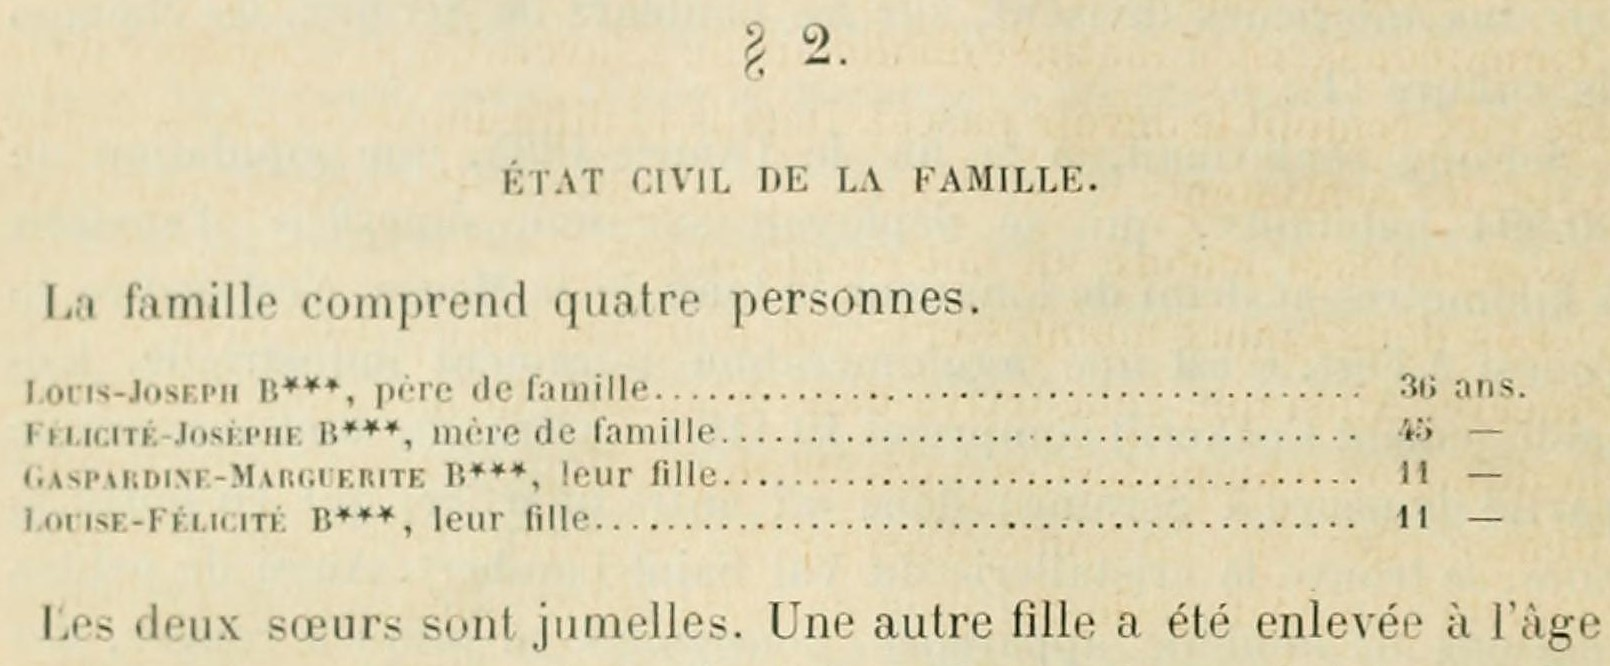
\includegraphics[width=14cm]{img/mono-56-page-4.jpg}
    \caption[Liste d'individus au début du paragraphe 2 (\no{} 56)]{Liste d'individus (série 2, volume 2, monographie \no{} 56, page 4).}
    \label{fig:mono-56-page-4}
\end{figure}

\begin{figure}[ht]
    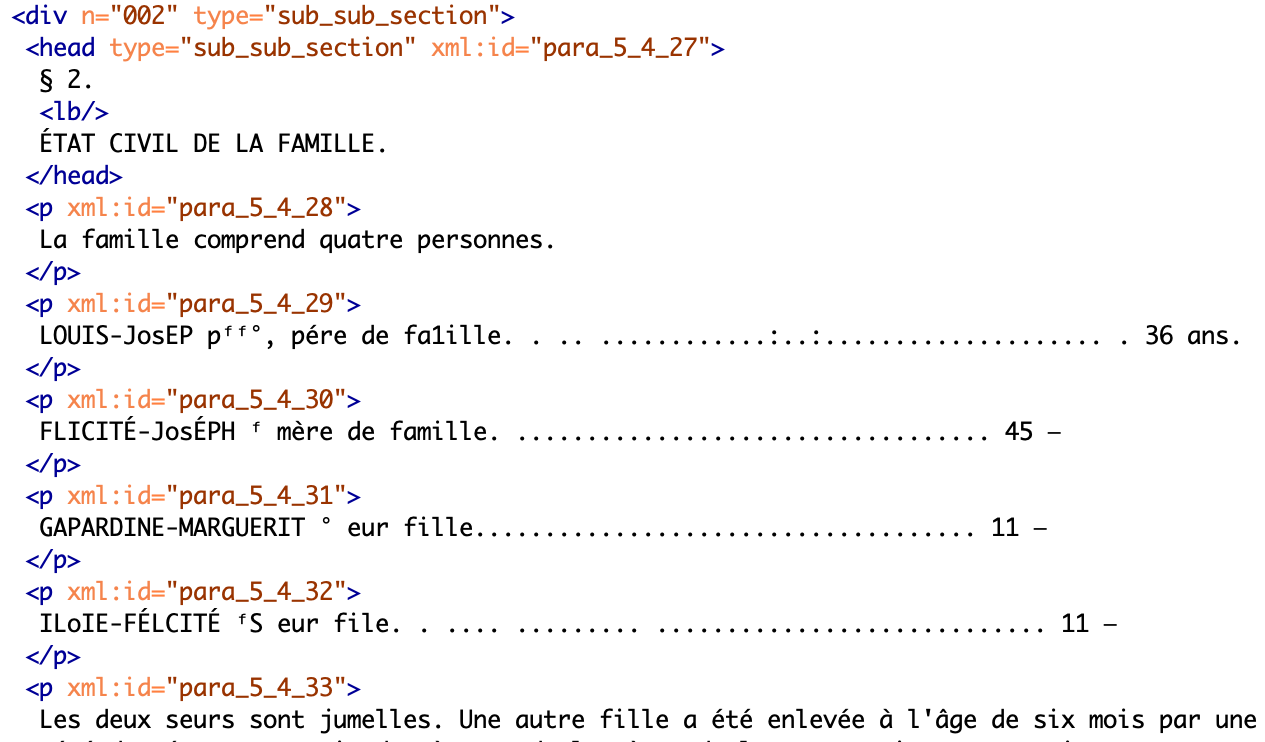
\includegraphics[width=14cm]{img/mono-56-page-4-code.png}
    \caption[Encodage de la liste d'individus (\no{} 56)]{Encodage de la liste d'individus, monographie \no{} 56 (\texttt{s2t2\_chapt\_5.xml}).}
    \label{fig:mono-56-page-4-code}
\end{figure}

Ici, ces erreurs ne posent pas qu'un problème de compréhension : elles empêchent la réalisation de la deuxième mission qui nous avait été confiée et qui consistait à lier les individus à leurs identifiants. En effet, cette opération se serait normalement traduite par l'implémentation d'une balise \texttt{<persName>} autour de chaque ensemble prénom et nom, avec un attribut \texttt{@ref} ayant pour valeur l'identifiant donné dans le fichier d'index.

L'implémentation automatique aurait pu s'effectuer de plusieurs manières, et notamment par la recherche du prénom : cela n'est pas possible du fait des distances d'édition trop grandes. Certaines monographies présentent également des listes numérotées (\fig{} \ref{fig:mono-23-page-209}) : là encore les numéros auraient pu être utiles, si seulement ils avaient été convenablement détectés.

\bigbreak

Une autre solution aurait procédé de l'observation que, les paragraphes deuxièmes commençant toujours par une phrase de type \og La famille comprend X personnes \fg{}, \og La famille comprend \fg{} ou \og Les membres de la famille sont \fg{}, les lignes qui suivent correspondent aux membres de la famille. Il eut été dès lors possible, grâce à l'ordre d'apparition noté dans le CSV, de considérer que la première de ces lignes est celle du premier individu, et ainsi de suite. Ce procédé repose cependant sur l'idée que les items des listes se trouvent sur une seule ligne, ce qui n'est pas toujours le cas (\fig{} \ref{fig:mono-23-page-209}). Du reste, placer une balise \texttt{<persName>} sur l'ensemble d'une ligne serait revenu à corrompre son usage, normalement réservé à \og un nom propre ou une expression nominale se référant à une personne \fg{}\footnote{\textit{TEI element persName (personal name)}, \textit{TEI Guidelines}.}.

Ainsi, dans tous les cas, la réalité des transcriptions empêchait l'implémentation automatique de la balise et nous confinait à une opération de correction.  Or celle-ci ne peut pas être menée sans une intervention humaine, qu'elle soit entièrement manuelle ou semi-automatisée grâce à un logiciel de suggestion de correction\footcite[p. 1]{sagot}. Ces logiciels --- par exemple, \textit{Antidote}\footnote{Présentation : \url{https://www.antidote.info/fr/} (consulté le \today).} --- s'appuient sur un lexique et, \og pour chaque mot inconnu, [cherchent] des candidats proches (par exemple en termes de distance d’édition) qui figurent dans le lexique et choisissent en prenant en compte la fréquence des candidats, le contexte, ou éventuellement un poids associé au type d’erreur présumé \fg{}\footcite[p. 1-2]{sagot}. Une telle intervention, quels que soient les moyens choisis pour sa réalisation, serait possiblement très longue et dans tous les cas coûteuse\footcite[p. 14]{en-tal}.


\begin{table}
\begin {center}
    \begin{tabular}{|c|c|c|}
\hline
    \textbf{Vérité terrain} & \textbf{\ocr} & \textbf{Correction} \\ \hline
    \textsc{Louis} & LOUIS & --- \\ \hline
    \textsc{Joseph} & JosEP & joseph \\ \hline
    \textsc{Félicité} & FLICITÉ & félicité \\ \hline
    \textsc{Josèphe} & JosÉPH & joseph \\ \hline
    \textsc{Gaspardine} & GAPARDINE & gagarine \\ \hline
    \textsc{Marguerite} & MARGUERIT & marguerite \\ \hline
    \textsc{Louise} & ILoIE & loin \\ \hline
    \textsc{Félicité} & FÉLCITÉ & félicité \\ \hline
    \end{tabular}
\caption{\label{tabl:pyspellchecker-1} Comparaison entre la vérité terrain, la transcription effectuée par l'\ocr{} et la proposition de correction de \texttt{pyspellchecker} pour les prénoms de la monographie \no{}~56 (série~2, volume~2, page~4 --- \texttt{s2t2\_chapt\_5.xml}).}
\end {center}
\end{table}

Nous nous sommes donc intéressés à la librairie Python \texttt{pyspellchecker}\footnote{Déposé sur \github{} :\url{https://github.com/barrust/pyspellchecker} (consulté le \today).}. Elle utilise un lexique, dont l'utilisateur spécifie la langue, et la distance de Levenshtein pour identifier des cacographies et proposer, selon les paramètres, soit une correction soit plusieurs candidats. La méthode \texttt{.unknown{}} affiche les mots du texte analysé qui ne se trouvent pas dans le lexique, et \texttt{.known()} ceux qui s'y trouvent\footnote{\texttt{Pyspellchecker} ne permet pas que de faire des corrections orthographiques ; en affichant les mots connus avec \texttt{.known()}, l'utilisateur peut calculer leur fréquence grâce à la méthode \texttt{.word\_probability()}.}. \texttt{Pyspellchecker} analyse ensuite les mots faux et peut, selon les paramètres, proposer une solution unique grâce à la méthode \texttt{.correction()} ou un choix entre plusieurs candidats grâce à la méthode \texttt{.candidates()}.  Par défaut, la distance est de \texttt{2}, elle peut être ramenée à \texttt{1}. Cela signifie que selon la valeur de la propriété \texttt{distance}, la librairie va considérer qu'une ou deux opérations de suppression, de substitution ou d'insertion ont pu avoir lieu.

Un test sur les cinq premiers \texttt{<p>} de la figure \ref{fig:mono-56-page-4-code} a donné de bons résultats (tabl. \ref{tabl:pyspellchecker-1}). Le script en question extrait le texte des balises \texttt{<p>} grâce à la librairie \texttt{BeautifulSoup} et le nettoie en enlevant les signes de ponctuation. Ces derniers induisent en effet le correcteur en erreur : un mot suivi d'un point sera ainsi considéré comme un seul ensemble et jugé faux\footcite[p. 60]{chiffoleau}. Le correcteur analyse ensuite chaque mot et retourne les mots faux ; nous l'avons paramétré de manière à ce qu'il propose une correction et des candidats de correction.

Le tableau \ref{tabl:pyspellchecker-1} montre que, sur sept transcriptions fausses, \texttt{pyspellchecker} permet d'en corriger quatre de manière exacte (\textit{Félicité} à deux reprises, \textit{Joseph} et \textit{Marguerite}). La vérité terrain est presque approchée pour \textit{Josèphe} : le \textit{e} final et l'accent grave manquent. En revanche, lorsque le même test est effectué sur une monographie où les prénoms ne se trouvent pas forcément dans un lexique français, par exemple la \no{} 25 consacrée à un parfumeur du bazar El Attharin-el-kebar de Tunis\footcite{mono025a}, le taux chute à un prénom corrigé sur sept erreurs (tabl. \ref{tabl:pyspellchecker-2}). La graphie de la vérité terrain \textit{Aïcha} figure bien dans la liste des candidats, mais c'est la forme \textit{Aisha} qui est choisie comme correction. On voit également que le dernier prénom, \textit{Kouka}, est transcrit avec une distance d'édition si importante (\textit{oul}, soit trois suppressions et une insertion) qu'il est improbable que le script puisse trouver le mot d'origine.

\begin{table}
\begin {center}
    \begin{tabular}{|c|c|c|}
\hline
    \textbf{Vérité terrain} & \textbf{\ocr} & \textbf{Correction} \\ \hline
    \textsc{Mohammed} & MloAMMED & mohammed \\ \hline
    \textsc{Kadidja} & bADIDJA & badidja \\ \hline
    \textsc{Rhkeïma} & Rhleima & rhleima \\ \hline
    \textsc{Ahsoûn} & Ahsoùn & ahsoka \\ \hline
    \textsc{Aïcha} & Aicha & aisha \\ \hline
    \textsc{Arouçi} & AroOuci & adouci \\ \hline
    \textsc{Kouka} & oul & oui \\ \hline
    \end{tabular}
\caption{\label{tabl:pyspellchecker-2} Comparaison entre la vérité terrain, la transcription effectuée par l'\ocr{} et la proposition de correction de \texttt{pyspellchecker} pour les prénoms de la monographie \no{}~25 (série~1, volume~3, page~286 --- \texttt{s1t3\_chapt\_10.xml}).}
\end {center}
\end{table}

Si ce test pourrait être transformé en un script d'aide à la correction, la présence d'un opérateur humain pour valider ou non les propositions de \texttt{pyspellchecker} reste indispensable. C'est la méthode utilisée par Floriane Chiffoleau (prom. 2019) lors de son stage de fin d'étude au sein du projet MetaLEX de l'EHESS, dont l'objectif est \og d’élaborer un système d’informations métalexicographiques,
concernant le vocabulaire portant sur les langues historiques du droit en Europe \fg\footcite[p. 9]{chiffoleau}. Elle a plus précisément travaillé sur l'édition numérique du \textit{Dei Delitti e delle Pene} de Cesare Beccaria (1764), ce qui l'a conduit à utiliser \texttt{pyspellchecker} pour corriger les résultats de son \ocr. Elle produit dans son mémoire un retour d'expérience détaillé sur l'utilisation de cette librairie, en insistant sur la division des tâches et la constitution de dictionnaires Python\footcite[chap. 8, \textit{Établir une correction orthographique et une annotation linguistique semi-automatique}, p. 57-66]{chiffoleau}.

Cinq étapes sont décrites. La première consiste à nettoyer et mettre en forme automatiquement le texte en supprimant les sauts de ligne, les espaces en trop et les signes de ponctuation\footcite[p. 54 et 60]{chiffoleau}. Les erreurs sont ensuite relevées par \texttt{pyspellchecker} et réparties en trois ensembles : une liste avec les mots non-reconnus mais justes, un dictionnaire Python avec les versions non-usuelles du \textsc{xvii}\ieme~siècle (par ex. \textit{paroître} à la place de \textit{paraître}\footcite[p. 57]{chiffoleau}) et un dernier dictionnaire contenant les erreurs véritables et leurs corrections\footcite[p. 59-60]{chiffoleau}. Lors de la troisième étape, le texte est cette fois-ci récupéré en entier, avec sa mise en forme et sa ponctuation\footcite[p. 61]{chiffoleau}. Le dictionnaire d'erreurs est passé en revue lors de l'étape suivante afin de contrôler et d'amender si nécessaire les propositions de \texttt{pyspellchecker}\footcite[p. 61-63]{chiffoleau}. Les opérations de correction sont enfin opérées à l'aide d'une fonction de recherche et de remplacement à partir du dictionnaire d'erreurs : chaque mot faux est recherché et ses occurrences sont remplacées par sa correction\footcite[p. 63-64]{chiffoleau}.

\texttt{Pyspellchecker} a  fait ses preuves dans plusieurs projets de recherche : MetaLEX, comme nous venons de le voir, mais également DAHN pour lequel Floriane Chiffoleau travaille aujourd'hui en tant qu'ingénieure de recherche et de développement de l'équipe ALMAnaCH. Son expérience et ses scripts peuvent être ré-utilisés pour les fichiers des \odm{}, avec quelques modifications dues notamment au fait que nos fichiers ne contiennent pas de mots en ancien français\footnote{Les scripts utilisés par Floriane Chiffoleau lors de son stage sont déposés sur \github{} : \url{https://github.com/FloChiff/memoire-M2/tree/master/Livrable\%20technique/Scripts/2\%20-\%20Nettoyage\%20de\%20texte} (consulté le \today).}. Nous pouvons également observer que la majorité du processus est automatisé, mis à part la correction du dictionnaire d'erreurs.

Une autre librairie Python, \texttt{pygrammalecte}, peut être utilisée pour générer un rapport d'identification des erreurs. La différence avec la librairie précédente est qu'elle fonctionne avec un dictionnaire et est capable, en plus de détecter les erreurs, de les répartir dans une typologie (orthographe, grammaire, ponctuation). Cette librairie est utilisée par le service humanités numériques de l'École nationale des chartes pour évaluer la qualité des \ocr{} des positions des thèses pour le diplôme d'archiviste paléographe, et permet de générer un rapport d'erreur sous la forme d'un fichier JSON\footnote{Voir notamment la fonction \texttt{ocrquality} dans le script \texttt{encpos\_control.py}, ligne 72 : \url{https://github.com/chartes/encpos/blob/38ad0277a03467642dd8a329a37237c9e663f4d1/utils/encpos_control.py\#L72} (consulté le \today).}.

On le voit, il est possible de développer des solutions en interne pour corriger une \ocr. Si elles n'automatisent pas totalement cette correction, elles permettent de réduire son coût budgétaire en épargnant le recours à un prestataire externe ou l'achat d'un logiciel dédié. Elle peuvent néanmoins se traduire par le recours à un vacataire pour le temps de la correction, ce qui représente tout de même un poste de dépense.

Durant notre stage, nous avons contourné le problème en ajoutant, au début des deuxièmes paragraphes, un commentaire contenant les identités des individus cités et leurs identifiants. Un commentaire est dans un fichier informatique une section du code destinée à la lecture par un humain et non par une machine, qui de fait l'ignore au moment de l'interprétation du fichier. En XML, le commentaire est délimité par les symboles \texttt{<!--} et \texttt{-->}. Dans la monographie \no{} 56, cela donne cette ligne :

\begin{quote}
    \texttt{<!-{}- Individus cités : Louis-Joseph B*** (\no{}056aE1) - Félicité-Josèphe B*** (\no{} 056aE2) - Gaspardine-Marguerite B*** (\no{} 056aE3) - Louise\-Félicité B*** (\no{} 056aE4) -{}->}
\end{quote}

Il s'agit d'une solution d'attente qui n'a pas vocation à demeurer dans la version définitive des fichiers.

\chapter{Une valorisation plurielle}

\section{Édition papier, édition numérique}

Un postulat commun veut qu'une édition numérique offre à son utilisateur plus de possibilités qu'une édition papier n'en offre à son lecteur\footnote{\og \textit{Often these descriptions glance at their print predecessors, usually with expressions of how much more these digital editions can contain than ever could be included in print editions, and how much more the reader can do with them} \fg{} : \cite[p. 105-106]{robinson}.}. Le numérique permet en effet de concevoir des plate-formes sur mesure pour la consultation des textes, et les outils des humanités numériques permettent à \og de nombreuses données non interrogeables jusqu’à présent [d'être] l’objet d’enquêtes \fg\footcite[p. 20]{duval}. \og Des structures cachées, des faits de système difficilement décelables à l’œil et à la main \fg{} deviennent ainsi accessibles\footcite{duval}.

Dans le programme \timeus{}, l'édition numérique des \odm{} a éveillé l'intérêt d'au moins trois participants. Le LARHRA de l'université de Lyon 2, dans le strict respect des objectifs du programme, souhaite utiliser les informations économiques fournies par les tableaux de budget et celles d'ordre prosopographique contenues dans le paragraphe \og §2 --- État civil de la famille \fg. L'équipe ALMAnaCH d'Inria a pour sa part la volonté de puiser dans les champs lexicaux des mondes ouvrier et industriel afin d'alimenter des algorithmes de traitement automatique du langage (TAL). Enfin, le Centre de recherches historiques (CRH) veut fournir à la communauté scientifique une édition numérique des \odm{} qui intégrerait des informations matérielles sur la constitution du corpus et le travail de la \sess.

On le voit, les objectifs poursuivis par ces entités sont très divers. Les matériaux qui permettront de les réaliser le sont tout autant : le LARHRA et ALMAnaCH ont besoin de données brutes issues des tableaux statistiques (des chiffres) et du texte (des mots), tandis que le CRH agrège des métadonnées inédites qui proviennent de plusieurs corpus ; il dispose notamment d'un exemplaire des deuxième et troisième séries encore à l'état de fascicules non reliés. Le LARHRA a également besoin d'une transcription de qualité pour s'assurer de la viabilité des informations prosopographiques du second paragraphe.

Cette pluralité de directions illustre la tension qui traverse les éditions numériques : elles portent avant tout sur un document et non sur une \oe{}uvre\footnote{\og \textit{Two decades of making digital editions, and recent papers about digital editions, have moved the needle away from the “work” to the “document”, to the point where we might need only think of “documents”} \fg{} : \cite[p. 107]{robinson}}. Cette distinction est issue de la triade document, texte, \oe{}uvre (\textit{document}, \textit{text}, \textit{work}) qui désigne les dimensions matérielle, linguistique et intellectuelle d'un écrit\footnote{\og \textit{Work} désigne le texte de l’auteur, éventuellement le texte correspondant à la volonté de l’auteur, et implique la notion d’authenticité ; \textit{text} dénomme la séquence linguistique attestée dans un document transmettant l’œuvre ; enfin \textit{document} est une manifestation physique d’un text \fg{} : \cite[p. 15-16]{duval}.}. De fait, l'encodage que nous avons décrit dans la partie précédente fait la part belle au document \odm{} de l'Université de Toronto, digitalisé par \ia. \transkribus{} et le script \lse{} mobilisent la TEI pour conduire sa reproduction fidèle grâce à des ensembles \texttt{<facsimile>}\footcite[p. 124]{robinson}. L'\oe{}uvre n'est pas pour autant oubliée. Elle se rencontre dans la structure logique leplaysienne, là encore reproduite fidèlement par le biais des divisions et des titres.

Cette coexistence apparente et inégale n'a cependant pas vocation à durer : dans la vision de \timeus, c'est bien l'\oe{}uvre et non le document qui doit prendre le dessus. Il n'est pas question de concevoir un support de consultation qui présenterait des échantillons successifs correspondant au contenu d'une page. Cela reviendrait à reproduire l'interface de visualisation d'\ia, tout en donnant une réalité concrète à l'hypertexte qui est \og en gestation dans les tables, index et diverses aides à la lecture de consultation déjà présentes \fg{} dans les volumes\footcite[p. 19]{duval}.

Ces observations montrent qu'une édition numérique se doit d'être équilibrée et de rendre compte à la fois du document-texte et de l'\oe{}uvre-texte\footnote{\og \textit{A scholarly edition must, so far as it can, illuminate both aspects of the text, both text-as-work and text-as-document} \fg{} : \cite[p. 123]{robinson}.}, sans quoi elle risque de perdre tant ses lecteurs\footnote{\og \textit{But there are dangers here. (...) Facsimile editions in print form are of very little use to the reader, or even to scholars, whose interest (...) is likely to be in questions of how the received text changed over time, how it was received, how it was altered, transformed, passed into different currencies. If we make only digital documentary editions, we will distance ourselves and our editions from the readers} \fg{} : \cite[p. 127]{robinson}.} que ses utilisateurs\footnote{\og La lisibilité des éditions électroniques n’a rien à envier à celle des éditions papier. (...) Parfois, les interfaces ne sont pas intuitives et requièrent une longue familiarisation ; d’autres fois, des aides à la lecture systématiquement présentes dans les éditions papier disparaissent \fg{} : \cite[p. 21]{duval}.}.

Le premier essai d'édition des fichiers XML, mené par Alix Chagué, consiste ainsi en un document HTML où l'intégralité du texte du premier volume est reproduit, organisé en fonction de la structure logique et non des zones de segmentation\footnote{Cette démonstration est visible à cette adresse : \url{http://demo-leplay.herokuapp.com/volume_parsed_test.html} (consulté le \today).}. Elle pourrait cependant être améliorée avec des informations issues du document, à commencer par la traduction, par exemple entre crochets droits, des balises \texttt{<pb>} à chaque changement de page.

\timeus{} a identifié deux voies possibles pour une publication effective. La première consiste à déposer les textes sur \wikisource. Il s'agit d'une bibliothèque numérique maintenue par la fondation Wikimédia, gratuite, en \openaccess, contenant des \opendata{} (aucune restriction sur l'usage des données) et ouverte à tous ceux qui souhaitent y contribuer. Le problème est que les fichiers XML ne peuvent pas être versés en l'état : ils doivent être modifiés voire transformés dans la syntaxe de la Wikimedia, le wikicode. Cette opération peut donc s'avérer coûteuse et le transfert de la totalité des informations n'est pas garanti ; les dépôts git sont de ce \pov{} de bien meilleures solutions.

Cependant, le principe de \wikisource{} pourrait être conservé tout en contournant les règles de sa communauté. Le CRH souhaite en effet utiliser l'un de ses wikis sémantiques, \textit{Ethnocomptabilités}, pour publier les monographies et leurs métadonnées entendues au sens large (volumes, enquêtés, enquêteurs)\footnote{\textit{Ethnocomptabilités} est hébergé à cette adresse : \url{http://ethnocompta.huma-num.fr/} (consulté le \today).}. Un wiki sémantique est un wiki --- \cad{} une application web où des pages peuvent être créées et modifiées par des utilisateurs --- augmenté de renseignements sémantiques permettant de qualifier les relations entre les pages et, \textit{in fine}, de manipuler les données qui s'y trouvent\footcite{poupeau}. Le programme \timeus{} y est libre de publier ses données sous la forme qu'il souhaite ; cette publication doit néanmoins s'accompagner d'un effort de référencement et de communication afin que le wiki soit consulté et utilisé par la recherche.

\section{Retrouver les fascicules dans le volume}

Au premier abord, il est aisé de considérer les \odm{} comme une \oe{}uvre. Mais plus on progresse dans l'histoire de cette entreprise, plus cette idée première se fragilise. En effet, si ce corpus s'incarne aujourd'hui dans des volumes, ceux-ci étaient autrefois des fascicules. Il est en outre constitué de monographies réparties en trois séries, tout en formant un ensemble cohérent dont les membres \og prennent sens les uns par rapport aux autres \fg{}\footcite[p. 5]{chenu}. D'une certaine manière, la volonté du CRH d'explorer l'histoire matérielle du corpus pour compléter les métadonnées des fichiers XML remet en question l'existence de \og l'\oe{}uvre \odm{} \fg{}.

Les enjeux de l'édition numérique d'un texte imprimé aux \textsc{xix}\ieme{} et \textsc{xx}\ieme~siècles divergent de ceux sous-entendus par l'édition de texte imprimé lors de siècles antérieurs. Aucune ré-impression n'est ici attestée : le texte est le même d'un exemplaire à l'autre, et ce jusque dans ses imperfections. C'est la raison pour laquelle l'encodage ne fait aucun effort de lématisation et qu'il s'appuie, de fait, sur les seules numérisations des exemplaires de Toronto.

Dans l'encodage d'un texte imprimé tel que \lodm{}, le défi se situe non pas au niveau du texte et de ses différentes versions, mais bien dans la restitution de la génétique matérielle qui a amené à la constitution des volumes. Comment traduire dans l'encodage les stratégies mises en place par les différents relieurs pour fondre les fascicules dans le volume ? Dans les exemplaires de la Bibliothèque nationale de France, les feuillets liminaires des fascicules ont été placés après les tables, là où ailleurs ils ont été conservés dans le flux du texte. Il y a ici une subtilité dont l'encodage de niveau \og document \fg{} ne se préoccupe pas, et qui pourtant est essentiel pour les deux autres niveaux.

Les observations relevées par le CRH peuvent être insérées dans la partie \texttt{<sourceDesc>} du \texttt{<teiHeader>}. Le document encodé y est décrit dans une section \texttt{<msDesc>}, où une unité codicologique distincte de l'unité documentaire principale peut être elle-même décrite grâce à la sous-section \texttt{<msPart>} (\fig{} \ref{fig:tree_msDesc}).

\begin{figure}
    \centering
    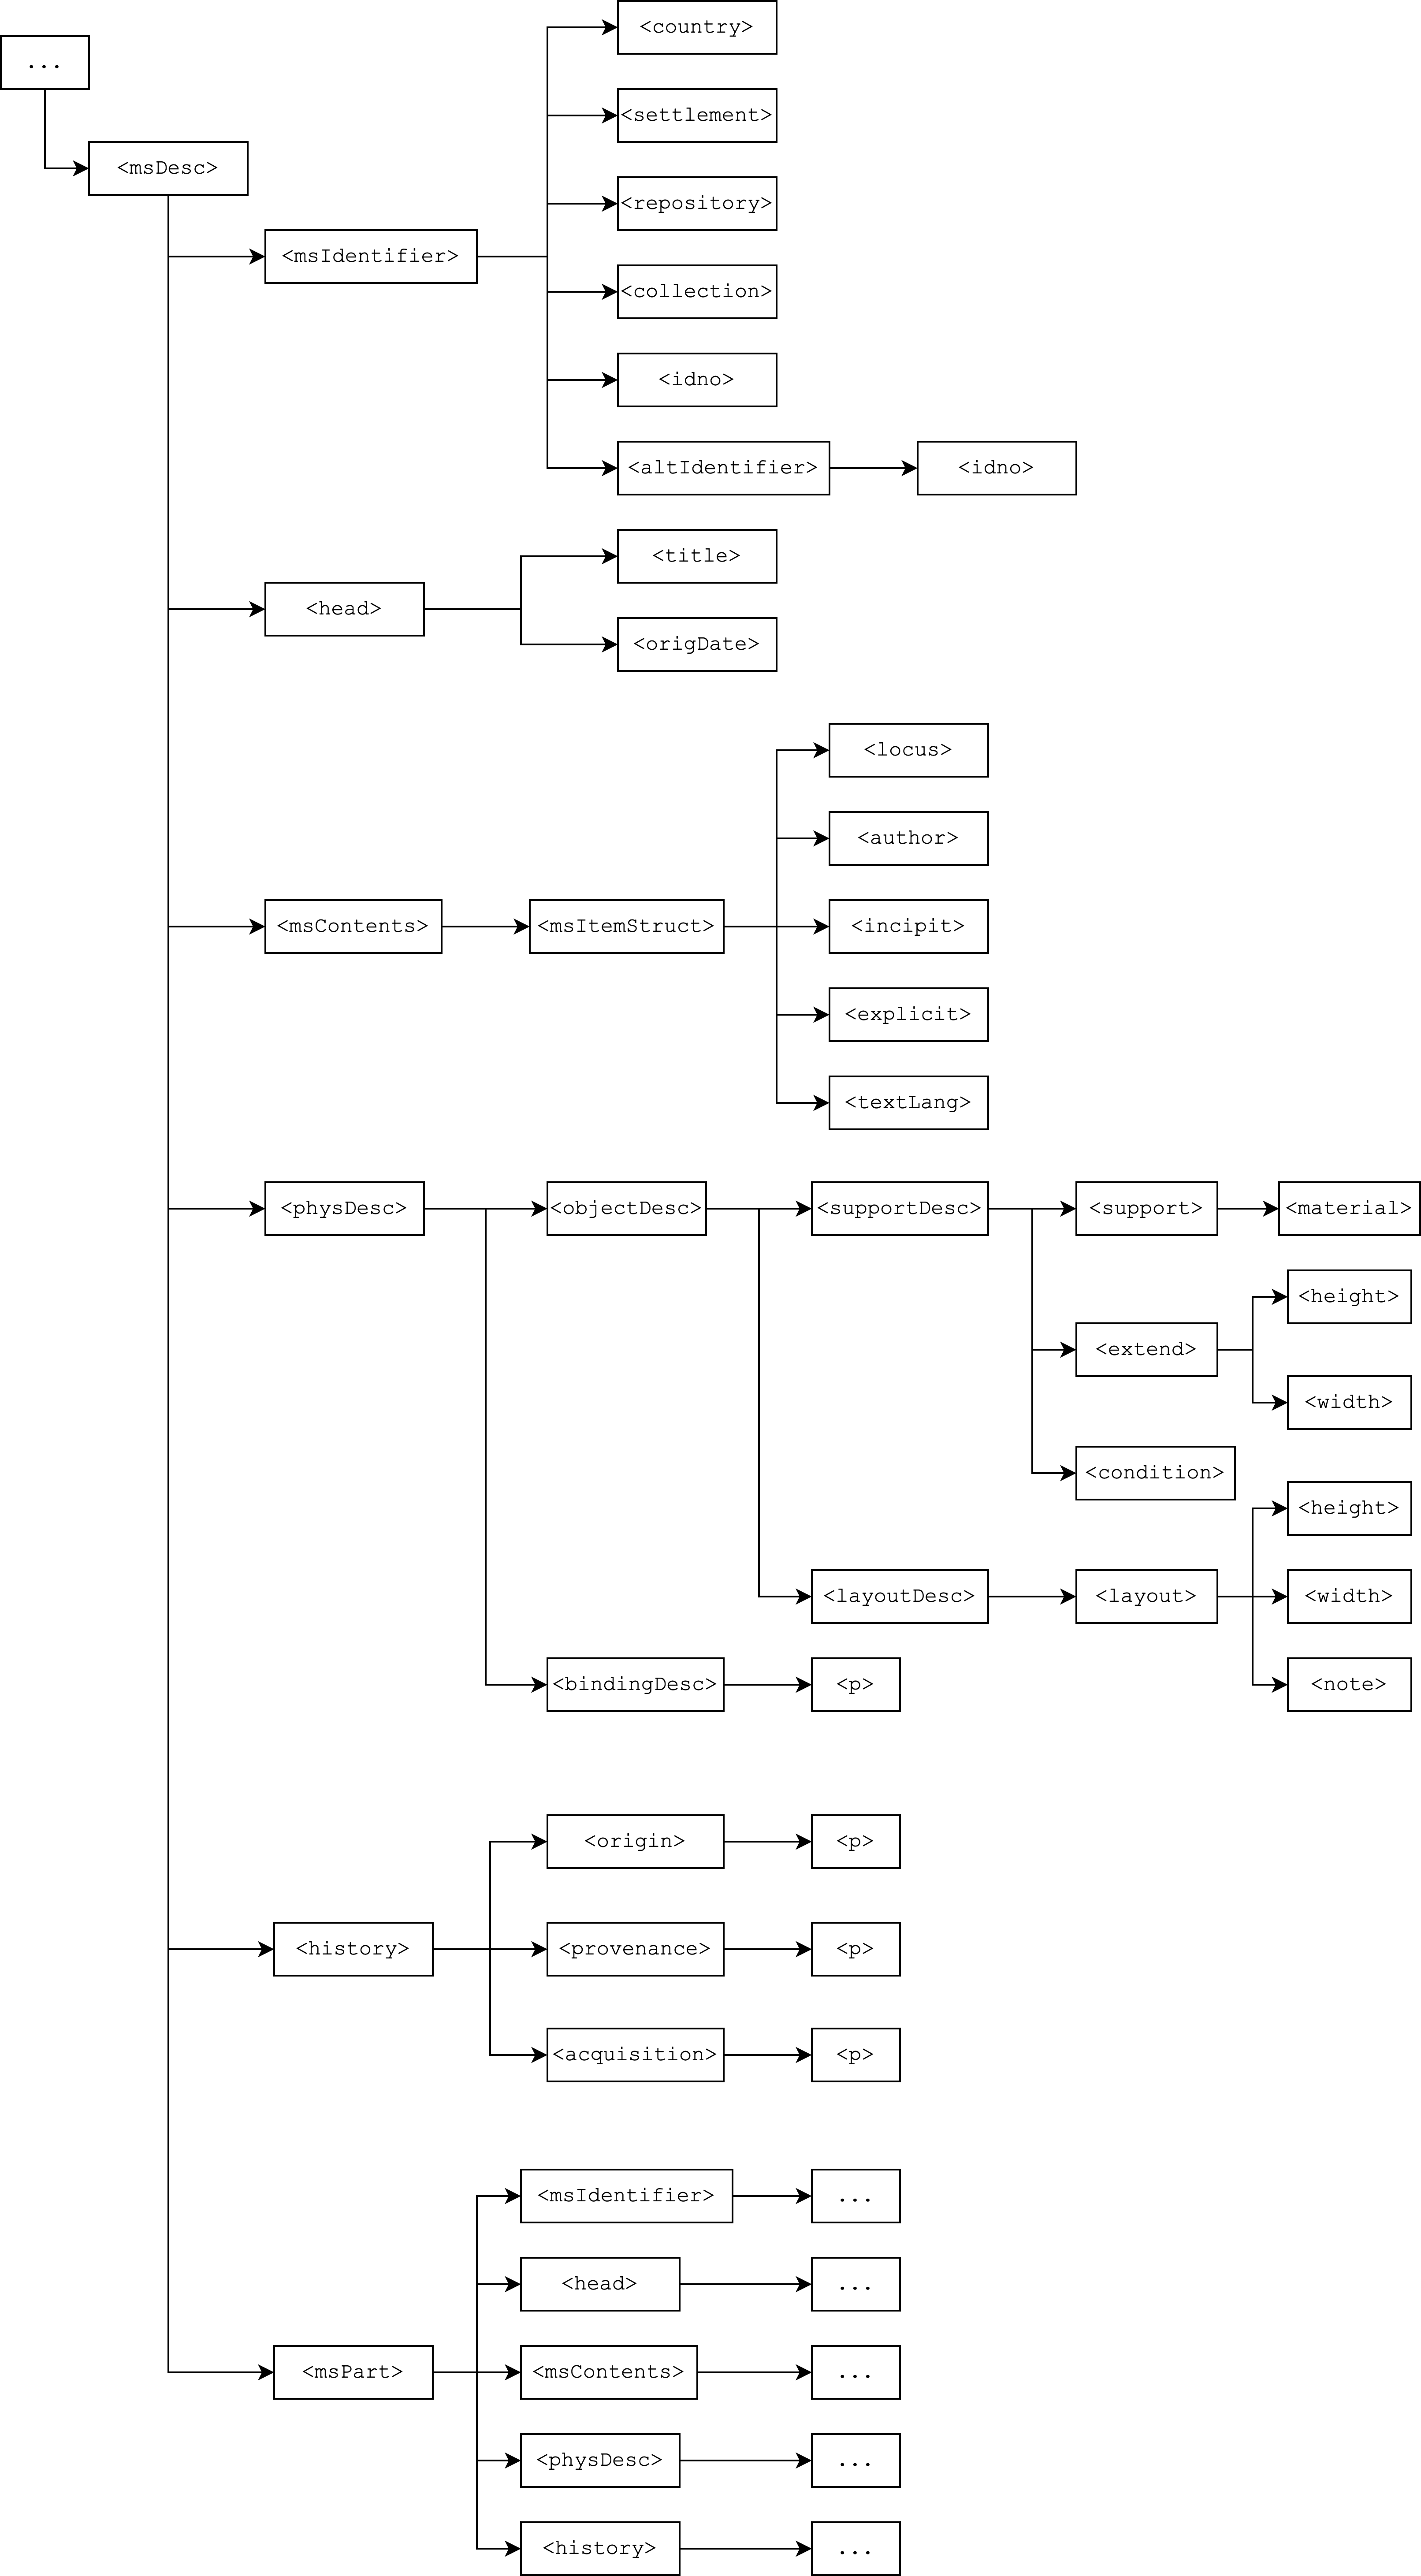
\includegraphics[scale=0.625]{img/tree_msDesc.png}
    \caption{Représentation de la section \texttt{<msDesc>} du \texttt{<teiHeader>}.}
    \label{fig:tree_msDesc}
\end{figure}

Plusieurs types de métadonnées sont spécifiés dans le \texttt{<msDesc>}. Le volume est tout d'abord identifié dans le \texttt{<msIdentifier>} par l'exposé de ses situations géographique (pays et ville de conservation) et institutionnelle (institution et département de conservation, cote), et la liste de ses copies, telles que la numérisation sur \ia. Il est ensuite titré et daté dans une partie \texttt{<head>}, avant que le \texttt{<msContents>} ne donne des informations sur sa structure : l'auteur, la pagination, la langue, l'\textit{incipit} et l'\textit{explicit}. Les caractéristiques physiques sont ensuite inscrites dans le \texttt{<physDesc>} (support, dimensions, mise en page, état). La reliure du volume et les marbrures des gardes sont décrites dans le \texttt{<bindingDesc>}.

L'histoire du volume est enfin détaillée dans la partie \texttt{<history>}, grâce à des éléments sur son origine (contexte d'édition), sa provenance (évènements entre l'origine et l'acquisition) et son acquisition (contexte d'acquisition). La pertinence d'une telle partie n'est pas certaine, tant pour les \odm{} que pour le corpus de fascicules non-reliés à la disposition du CRH et du CMH, car leurs histoires ne sont pas connues. Quelques relevés peuvent permettre d'éclaircir des points très spécifiques, par exemple la dédicace d'un monographe dans le volume 5\footnote{\og M. Auguste Moussel, hommage en cordial confraternité. Urbain Guérin \fg{} : \cite{mono083a}.}.

Le \texttt{<msDesc>} se conclurait par un \texttt{<msPart>} centré sur le fascicule, divisé selon le même plan.

Ces apports se bornent aux métadonnées, l'encodage produit par \lse{} et amélioré par notre reprise n'étant pas affecté. Rappelons que celui-ci n'est pas pour autant fixé. La place des objets graphiques reste à définir. Si la structure logique est en place, le système des renvois entre les monographies n'a pas été valorisé ; les informations prosopographiques doivent également être repérées et signalées après une correction des transcriptions.

\section{\textit{Quid} de la donnée ?}

Une question demeure au sujet des fichiers des \odm{} : quel avenir pour eux, non pas dans une mise en scène quelconque, mais en tant que données brutes ? Le choix de recourir au format XML-TEI montre que \timeus{} entend assurer la conservation des fichiers. La TEI est en effet maintenue par une communauté active. En rédigeant une cartographie du corpus et surtout une ODD, nous avons documenté la pratique éditoriale et favorisé sa compréhension par d'autres chercheurs et chercheuses ou projets qui souhaiteraient réutiliser l'encodage. Le dépôt en ligne sur le \gitlab{} de l'Inria assure la conservation de l'historique de nos interventions.

Néanmoins, le dépôt \gitlab{} est aujourd'hui en accès restreint, aussi le corpus n'est-il pas en accessible librement (\openaccess). Cette restriction est bien évidemment due au fait que le travail n'est pas achevé et sera levée à la fin du programme ANR. Pour autant, \timeus{} souhaite démultiplier les espaces de conservation en clonant le dépôt \gitlab{} sur \github. Ces deux sites offrent des services d'hébergement utilisant la technologie git, à la différence que \github{} est une entreprise commerciale possédée par Microsoft, aussi ne dépend-t-elle pas d'une institution publique dont les orientations budgétaires peuvent changer. Des procédures de migration existent entre les deux plates-formes et concernent les \commits{} comme les \issues{} et les \mergerequests.

Le CRH veut également verser les fichiers XML et peut-être, par sécurité, les images, dans l'entrepôt de données de l'EHESS, \textit{Didomena}\footnote{\textit{Le projet Didomena : une plate-forme moderne au service de la gestion des données de la recherche en sciences humaines et sociales} (\url{https://didomena.ehess.fr/informations}, consulté le \today).}. Cette application traite les données sur deux niveaux. Le logiciel \textit{Hyrax} reçoit d'abord les fichiers, les stocke et leur agrège des métadonnées dont les descriptions respectent le standard \textit{Portland Common Data Model}\footnote{Présentation accessible à \url{https://github.com/duraspace/pcdm/wiki} (consulté le \today).} ; elles sont ainsi assurées d'être interopérables. La seconde dimension est la couche applicative, soutenue par le logiciel \textit{Solr}, qui organise des vues logiques et permet des recherches à facettes dans les données comme dans les métadonnées. Le point faible est que la consultation n'est pas libre : il faut disposer d'un compte dans un établissement d'enseignement supérieur ou de recherche pour se connecter sur la plate-forme.

Ces différentes pistes montrent que les données des \odm, déjà standardisées, documentées et pérennisées, bientôt en \textit{open access}, sont assurées d'être indépendantes de toutes les mises en scène auxquelles elles pourraient se prêter\footcite[p. 63]{jolivet}.

Ces dernières années, l'écosystème de la donnée s'est néanmoins tourné vers la mise en relation de celles-ci\footcite[p. 66]{jolivet}. Une des conditions pour réaliser cela est l'interopérabilité. Les fichiers des \odm{} satisfont-ils à cette demande ? En d'autres termes, la question est de déterminer si les données qu'ils contiennent peuvent être enrichies par des informations venues d'autres formats, ou bien si elles peuvent être réutilisées par des programmes de recherche ou avec d'autres corpus dont le standard n'est peut-être pas la TEI, ou qui n'ont pas le même usage de la TEI. C'est là où le bât blesse : la TEI, du fait de son extrême souplesse, permet des pratiques éditoriales qui peuvent être très éloignées. Ce que les corpus gagnent en précision et en fidélité par rapport au(x) document(s) d'origine, ils le perdent en interopérabilité\footcite[p. 61-62]{jolivet}.

\newpage
\thispagestyle{empty}
\mbox{}
\newpage